\documentclass[../../tc_tp6_main.tex]{subfiles}

%\label{disenoCirc}
%\nameref{disenoCirc}

\begin{document}

%capítulo
\chapter{Oscilador de Wien}

\section{Introducción}

Se implementa un oscilador sinusoidal a partir de un circuito propuesto por la cátedra. Dicho oscilador tiene el nombre de ''Oscilador de puente de Wien'' y se basa en el criterio de Barkhausen para la oscilación de circuitos eléctronicos. A continuación se presentarán los principios básicos en los cuales se apoya el diseño del circuito. 
\subsection{Criterio de Barkhausen}

Sea un sistema realimentado. Este sistema cumple con la siguiente estructura: \par

\begin{figure}[H]	
	\centering
	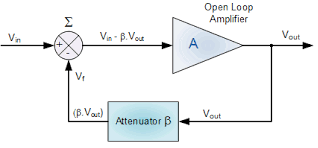
\includegraphics[scale=2]{imagenes/feedback_estructura.png}
	\caption{Estructura de general de un circuito con realimentación}
	\label{fig:ej1_feedback_estructura}
\end{figure}
El criterio de Barkhausen establece una condición necesaria (pero NO suficiente) para que  un circuito electrónico oscile.\par
Este criterio establece que dada una ganancia $A(s)$ para la etapa de amplificación de un circuito y dada la ganancia de realimentación del mismo, $\beta (s)$, entonces si $T = \beta (s)\cdot A(s)$ es la ganancia del lazo de realimentación del circuito, el mismo sólo podrá oscilar en su estado estacionario para aquellas frecuencias en las que se cumpla simultáneamente que: \par

\begin{itemize}
\item La ganancia de lazo sea unitaria, de manera tal que ${\displaystyle |T|=1\,}$. Este concepto se llama estabilidad neutra ya hay iguales cantidades de realimentación negativa que de positiva, es decir, ninguna prevalece por sobre la otra.
\item La fase de la ganancia de lazo $T$ tenga al mismo tiempo un valor múltiplo de $2\cdot k \cdot \pi$, con $k\epsilon \mathbb{Z}$
\end{itemize}

\subsection{Oscilador de Wien}

El oscilador de Wien es un oscilador que permite generar ondas senoidales en un amplio rango de frecuencias, sin ninguna señal de entrada. El oscilador cumple su función al lograr valores de resistencia dinámicos que afectarán a la ganancia de retroalimentación, logrando así cumplir el criterio de Barkhausen en tiempo estacionario y haciendo oscilar al sistema.\par

En particular, el oscilador requerido es de una frecuencia de 70kHz, por lo que habrá que tener consideraciones especiales a la hora de elegir el opamp con el que se trabajará además de los valores de los componentes.

\section{Presentación y análisis del circuito propuesto}

La cátedra propone el siguiente circuito:

\begin{figure}[H]	
	\centering
	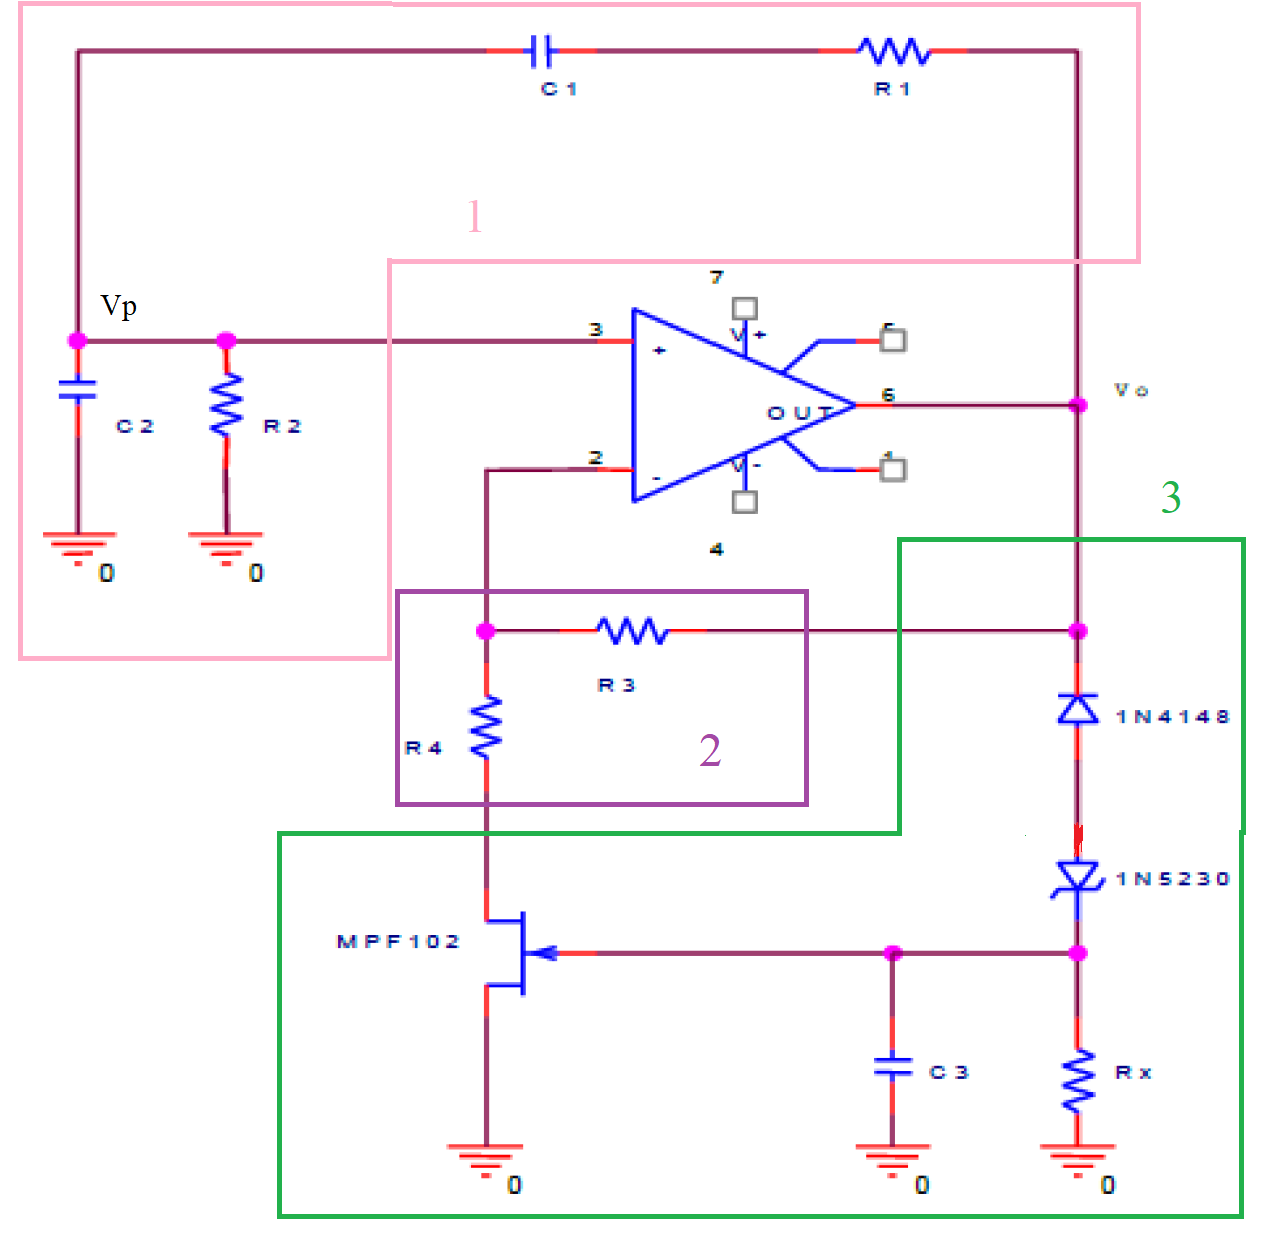
\includegraphics[scale=0.8]{imagenes/consigna_circuito.png}
	\caption{Circuito propuesto por la cátedra}
	\label{fig:ej1_consigna_circuito}
\end{figure}

donde se identifican las siguientes secciones a destacar: 

\begin{enumerate}
\item Realimentación positiva 
\item Realimentación negativa
\item Control automático de ganancia (CAG)
\end{enumerate}
\subsection{Análisis del subcircuito de realimentación}
\label{analsubreal}
	Los siguientes cálculos siguieron los pasos lógicos del libro de la cátedra, ''Design with Operational Amplifiers and Analog Integrated Circuits'' de Sergio Franco: \par
 Del circuito, se obtiene la siguiente relación por nodos: \par
 \begin{center}
 $\frac{V_\rho - V_o}{\frac{1}{s\cdot C_1}+R_1}= -V_\rho \cdot (s\cdot C_2 + \frac{1}{R_2})$
 	\end{center}
 	
 	De la cual se despeja el cociente: \par
 	
 	\begin{center} 
 	$\beta (s) = \frac{V_p}{V_o} = -\frac{C_1\cdot R_2 \cdot s}{C_1\cdot C_2\cdot R_1\cdot R_2 \cdot s^2 + (C_1\cdot R_1 + C_1\cdot R_2 +C_2\cdot R_2)\cdot s +1}$
 	\end{center}
 	Tomando, los valores de capacitancias y resistencias iguales de forma tal que $C_1 = C_2 = C$ y $R_1 = R_2 = R$, la expresión queda reducida a: \par
 	 \begin{center} 
 	$ \beta (s) = \frac{V_p}{V_o} = -\frac{C\cdot R \cdot s}{C^2\cdot R^2 \cdot s^2 +3\cdot C\cdot R\cdot s +1}$
 	\end{center}
 	\par Nótese de aquí que $\beta (s)$ tiene la forma de un pasabanda, con frecuencia central determinada por $\frac{1}{2\cdot \pi \cdot C\cdot R}$.\par
Por otro lado, la ganancia de realimentación negativa está dada por el no inversor entre las resistencias $R_3$ y  $R_4$:
	\begin{center} 
	$A(s) = 1+\frac{R_3}{R_4}$
	\end{center}
	 
	 Es de estas relaciones que se puede obtener la ganancia de lazo de realimentación, que está dada por $T(s) = A(s)\cdot \beta(s)$ y queda así determinada por: \par
	 \begin{center}
	 $T(s) =-\frac{(1+\frac{R_3}{R_4} )\cdot C\cdot R \cdot s}{C^2\cdot R^2 \cdot s^2 + 3\cdot C\cdot R\cdot s +1}$ 
	\end{center}
	Utilizando entonces el criterio de Barkhausen, se pide que para que el circuito al menos cumpla la condición necesaria de oscilación, la ganancia de lazo $T(s)$ tendrá que ser unitaria para la frecuencia de oscilación. Observamos cómo en la frecuencia central del pasabandas, $T(\frac{j}{C\cdot R}) = \frac{1+\frac{R_3}{R_4}}{3}$. Es así como si se lograra que $1+\frac{R_3}{R_4} = 3$ exactamente, se cumpliría simultáneamente que tanto $|T(\frac{j}{C\cdot R})| = 1$ como que la fase de $T(\frac{j}{C\cdot R})$ sea 0 grados, pudiendo así oscilar el circuito. \par
	En la práctica, hacer que los valores de resistencias y capacitancias se ajusten perfectamente a lo teórico es casi imposible, por lo que para solucionar este problema y así garantizar $1+\frac{R_3}{R_4} = 3$ exactamente, se utiliza un CAG (control automático de ganancia) que se encargará de regular la ganancia $1+\frac{R_3}{R_4}$ dinámicamente, haciéndola converger al valor esperado de 3. \par
	El CAG implementado en este circuito es con un transistor, que funcionará en su zona lineal como una resistencia variable dependiente de tensión. Esta resistencia estará en serie con la resistencia $R_4$, lo cual hará que variar la relación $\frac{R_3}{R_4}$ continuamente durante el funcionamiento del circuito, garantizando la oscilación del mismo. El control automático de ganancia y su implementación en este circuito será explicado en mayor detalle en la sección \nameref{cag}\par
	Se podrá obtener la transferencia total del sistema como $H(s) = \frac{A(s)}{1 + \beta (s) \cdot A(s)} = \frac{1}{\beta (s)} \cdot \frac{T(s)}{1+T(s)}$ \par
	
	\begin{center}
	$H(s) = \frac{(1+\frac{R_3}{R_4})\cdot (C^2\cdot R^2 \cdot s^2 + 3\cdot C\cdot R \cdot s+1)}{C^2\cdot R^2 \cdot s^2 + C\cdot R \cdot (\frac{R_3}{R_4}+4) \cdot s +1}$
	\end{center}
	
	Debe aclararse que la salida del oscilador puede ser tomada en $V_o$, pero que al ser tomada en $V_p$ la salida será más pura, es decir tendrá menor distorsión armónica. Esto se debe a que en $V_p$ se obtendrá la salida directa de haber filtrado a la señal por un pasabanda y por lo tanto se obtendrá una menor cantidad de componentes para otras frecuencias. El inconveniente de tomar la salida en $V_p$ es que para hacer esto se deberá utilizar un buffer para evitar que los circuitos conectados se carguen entre sí. Es por esto que se decidió tomar la salida en $V_o$ a expensas de obtener una peor distorsión armónica.
	

\subsubsection{Transistor JFET y curvas}
\label{curvas_trans}
Se hace un análisis mediante simulación de cómo varía la corriente Ids del transistor en función de la tensión de GATE del jfet y de la tensión Drain-Source. 

\begin{figure}[H]	
	\centering
	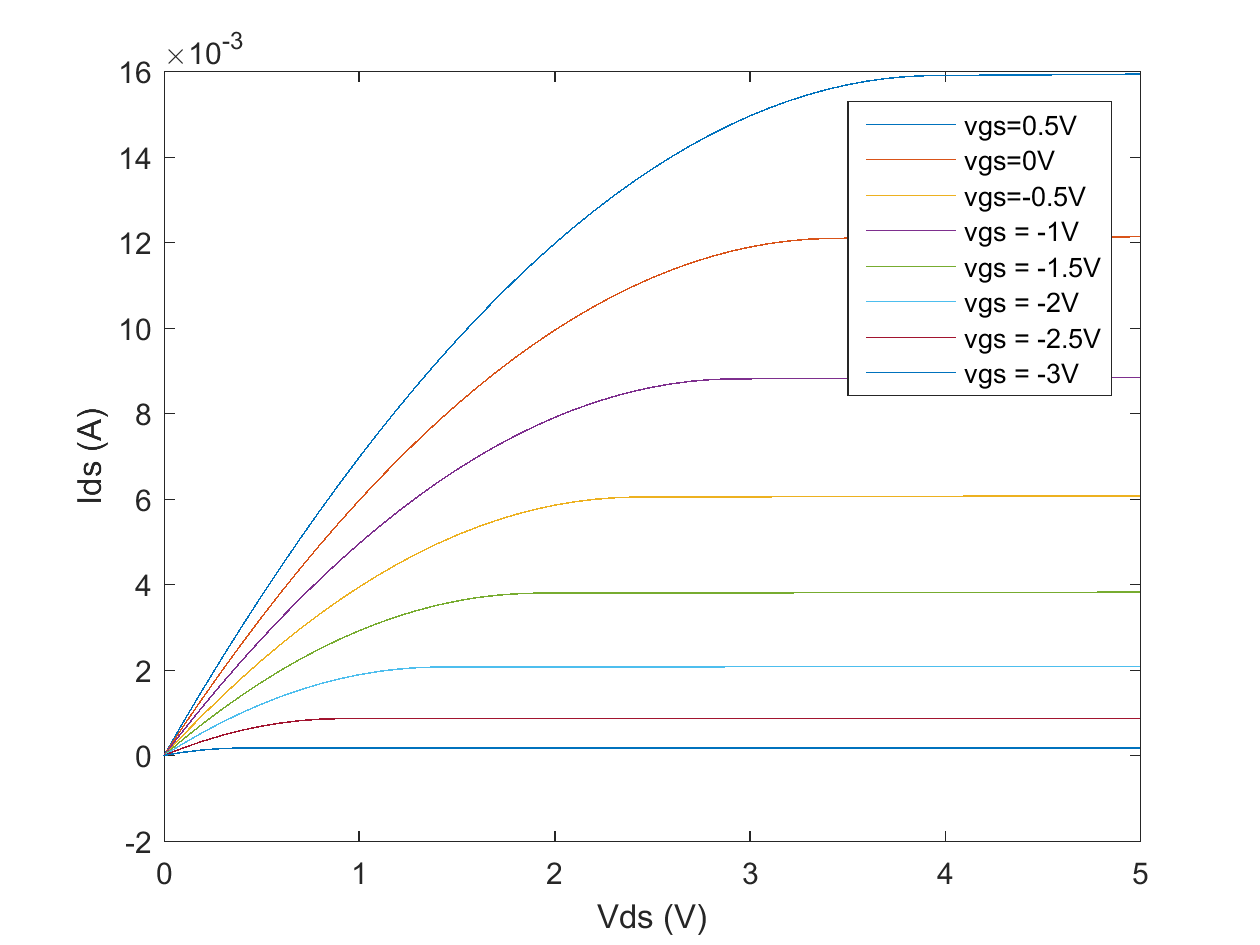
\includegraphics[scale=0.5]{imagenes/corrientes_jfet.png}
	\caption{Curvas de corriente del jfet MPF102}
	\label{fig:ej1_corrientes_jfet}
\end{figure}

\begin{figure}[H]	
	\centering
	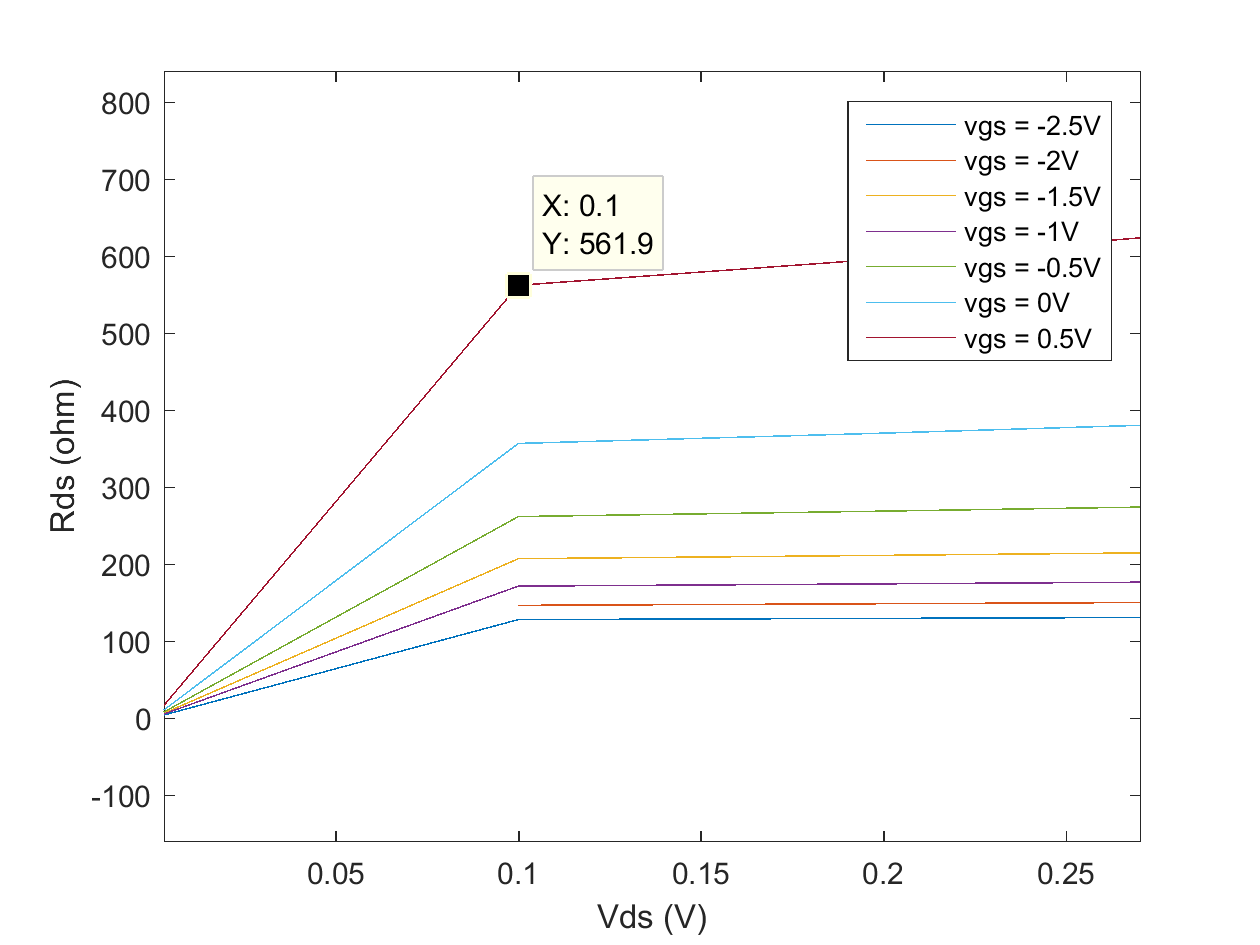
\includegraphics[scale=0.5]{imagenes/resistencias_jfet.png}
	\caption{Curvas de resistencias del jfet MPF102}
	\label{fig:ej1_resistencias_jfet}
\end{figure}

Se hace un enfoque en el rango -3V a -3.5V para Vgs porque se utilizará luego: 

\begin{figure}[H]	
	\centering
	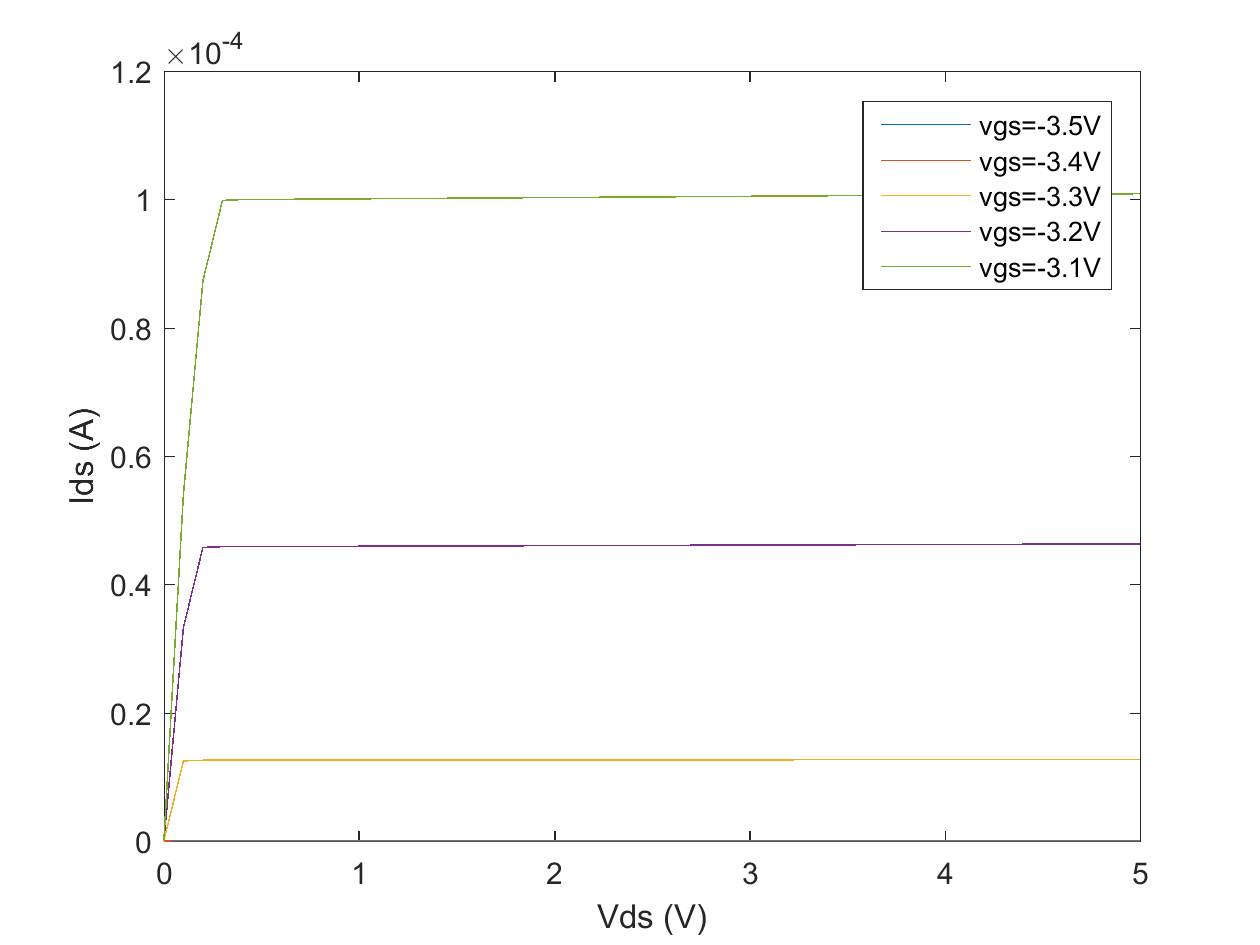
\includegraphics[scale=0.4]{imagenes/corrientes_jfet_vgs_bajo.png}
	\caption{Curvas de corriente del jfet MPF102}
	\label{fig:ej1_corrientes_jfet_vgs_bajo}
\end{figure}

\begin{figure}[H]	
	\centering
	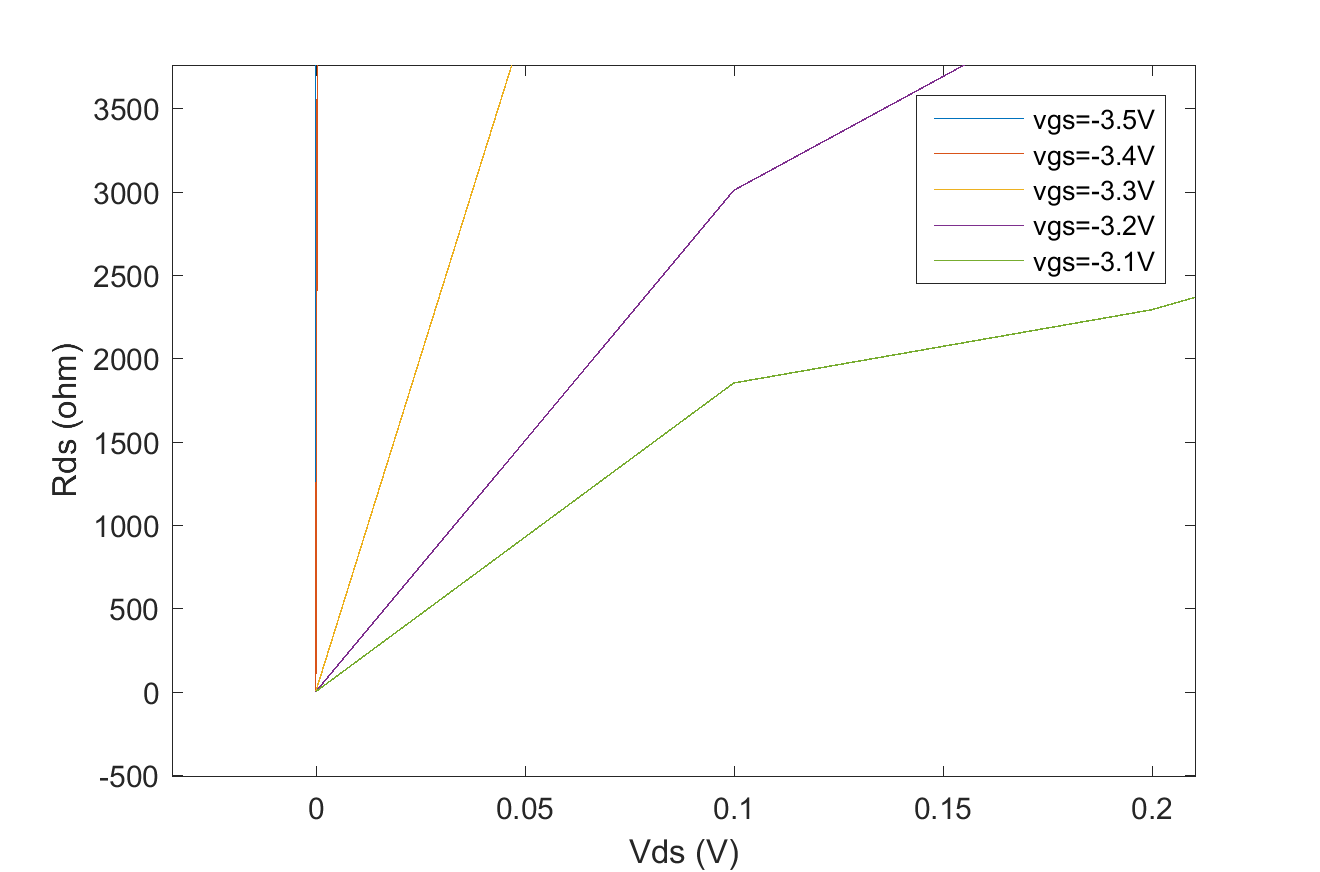
\includegraphics[scale=0.45]{imagenes/resistencias_jfet_vgs_bajo.png}
	\caption{Curvas de resistencias del jfet MPF102}
	\label{fig:ej1_resistencias_jfet_vgs_bajo}
\end{figure}

Como el p-channel tiene las tensiones invertidas con respecto al n-channel, se propone invertir a los diodos cuando se utiliza un p-channel, de tal manera que la tensión comience a subir en la realimentación e inmediatamente active al transistor, que terminará invirtiendo la tensión inicial y  así resultará en el mismo circuito anterior.

\subsection{Control automático de Ganancia (CAG)}
\label{cag}
	El control automático de ganancia pretende ajustar la ganancia de lazo a un valor exactamente unitario, evitando errores por tolerancias y resistencias agregadas en los capacitores no ideales y demás.\par
	Para esto se divide al CAG en las siguientes secciones:
	
	\begin{figure}[H]	
	\centering
	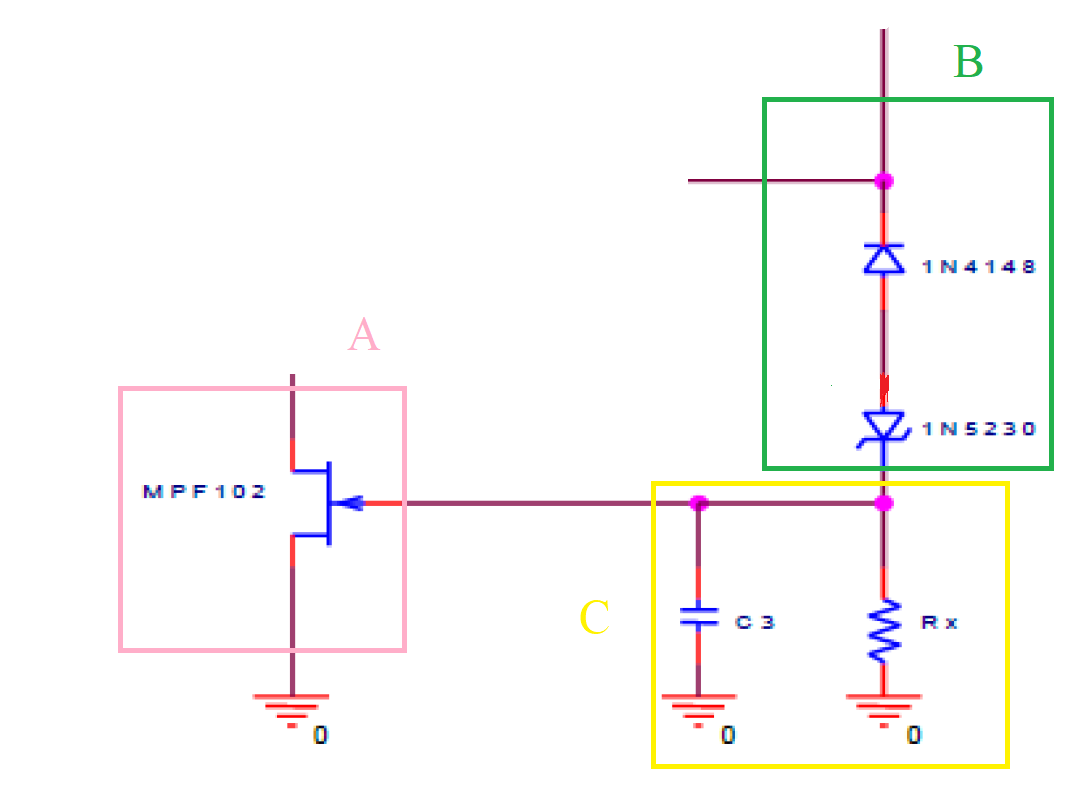
\includegraphics[scale=0.5]{imagenes/cag.png}
	\caption{Secciones del CAG}
	\label{fig:ej1_cag}
\end{figure}

\begin{enumerate}
\item $A$: Transistor como resistencia variable.
\item $B$: Switch on-off del transistor.  
\item $C$: Controlador de respuesta en frecuencia para los diodos.

\end{enumerate}

\begin{itemize}
\item \underline{Transistor como resistencia variable}:\par
El transistor trabajará en su zona lineal como resistencia, alterando así la relación $\frac{R_3}{R_4}$ y con ella la ganancia de lazo del circuito hasta que converga a la unidad par ala frecuencia de oscilación, como se mencionó anteriormente. De las curvas anteriores, se observa entonces que la tensión Drain-Source del transistor por lo tanto variará poco, entre los 0 y 0.1V para que el transistor opere siempre en su zona lineal (tensión Vds proporcional a Ids, por lo que el transistor equivale a una resistencia). \par
Los valores de tensión en el GATE del transistor son los que regularán cuál curva se tomará, y por ende el valor de resistencia que adopatará el transistor, convirtiendo efectivamente al transistor en una resistencia controlada por tensión.\par
Observamos de aquí que la mayor resistencia será para Vgs =0.5V, y la menor para tensiones Vgs negativas. Como el cambio de Vgs altera la curva que se utiliza, se hace notar que cambios abruptos de la tensión del GATE implicarán cambios abruptos en la resistencia del transistor, pudiendo así tener picos de alta pendiente en tensión y consecuentemente alinealidades no deseadas. Es por esto que se intentará mantener el cambio de Vgs lo más chico posible, a modo de cambiar el valor de resistencia dinámicamente pero no de forma demasiado abrupta. \par
\item \underline{Switch on-off del transistor}:\par
Si se hace un análisis incremental del conciente $\frac{R_3}{R_4}$ a lo largo del tiempo, se requiere que el cociente al principio sea $\frac{R_3}{R_4} > 2$ a modo tal de que el circuito comience a ganar rápido en tensión a la salida para así comenzar con la oscilación. Luego, al llegar a algún valor límite, el transistor deberá activarse como resistencia a modo tal de disminuir  $\frac{R_3}{R_4} $ de tal manera que $\frac{R_3}{R_4} < 2$. Estas diferencias con la relación $\frac{R_3}{R_4} = 2$ deberán ser dispuestas de manera tal que eventualmente estas converjan al valor 2, cumpliéndose finalmente el criterio de BarkHausen.\par
Para lograr esto, se decide que con el transistor apagado (sin actuar como resistencia o con un valor de resitencia bajo), $\frac{R_3}{R_4} > 2$. El método de decisión de cuándo comenzará el transistor a jugar como resistencia lo definirán entonces los diodos del circuito: \par
En el momento en que la tensión obtenida supere un valor umbral en tensión definido por los diodos (4.7V del Zener + 0.7V del diodo = 5.4V), los diodos comenzarán a conducir, se cargarán entonces $C_3$ y $R_3$ y la tensión en Vgs por lo tanto cambiará de manera tal que se altere la relación  $\frac{R_3}{R_4}$ al aumentar la resistencia del transistor, de modo que $\frac{R_3}{R_4+R_t}<2$, donde $R_t$ representa la resistencia dinámica del transistor.\par
Al ser el umbral de cambio definido por los diodos, la amplitud de la oscilación luego de transcurrir el tiempo de establecimiento estará directamente relacionada a este umbral. Es así como en la simulación se podrá observar que la tensión pico resultante será cercana a 5.4 V.\par

\item \underline{Controlador de respuesta en frecuencia para los diodos}:\par
Como los diodos tienen un comportamiento no lineal, el cambio de tensión en el GATE resultante de superar la tensión umbral será abrupto y agregará componentes en frecuencia al circuito, algo no deseado para un oscilador senoidal. Además, la resistencia del transistor luego de haberse establecido el circuito deberá tener valores muy precisos, de modo tal que $\frac{R_3}{R_4+R_{tFinal}}=2$ exactamente, se requiere también que la tensión del GATE no varíe abruptamente . Aquí es donde entra en juego el capacitor $C_3$, que junto con $R_x$ limitarán la respuesta en frecuencia al formar un filtro pasabajos con constante de tiempo de carga $R_x\cdot C_3$ para el análisis transitorio. Como queremos que la variación de la tensión de GATE sea chica mientras el transistor está actuando como resistencia, pedimos que dicha constante de tiempo sea alta, por lo que valores altos para $R_x$ y $C_3$ cumplirán con el objetivo. Es importante destacar que si los valores no son lo suficientemente grandes, el circuito no oscilará por dos posibles motivos: 
\begin{enumerate}
\item La carga acumulada en el capacitor y la resistencia no serán suficientes como para alterar Vgs de modo tal que se obtenga la resistencia deseada en el transistor.
\item El capacitor se descargará antes de transcurrido el tiempo necesario para lograr estabilizar la ganancia, de manera tal que el transistor variará su resistencia erráticamente, no pudiendo así estabilizarse para la frecuencia requerida.
\end{enumerate}
\end{itemize}

\subsection{Amplitud de la oscilación}
Como se dijo previamente, la amplitud de oscilación está íntimamente relacionada con la la caída en tensión de los diodos.\par
Dado que los diodos fijan un valor umbral de tensión a partir del cual comenzarán a conducir y así el transistor comenzará a actuar como resistencia, variando la ganancia de lazo, se espera que el incluir una resistencia entre los diodos variará la amplitud al demandar mayor tensión para que se cumpla este umbral de transición. Se corrobora esto con simulación. \par
\begin{figure}[H]	
	\centering
	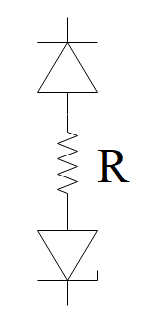
\includegraphics[scale=0.5]{imagenes/resistencia_diodos.png}
	\caption{Circuito modificador de amplitud propuesto}
	\label{fig:ej1_resistencia_diodos}
\end{figure}
Es así como introduciendo un preset entre diodos se podrá aumentar la amplitud de salida al retardar el punto en que el transistor llega al valor de resistencia estabilizador del circuito.\par
Introduciendo un preset entre los diodos se podrá lograr entonces aumentar la amplitud de la señal de oscilación resultante.\par

\begin{figure}[H]	
	\centering
	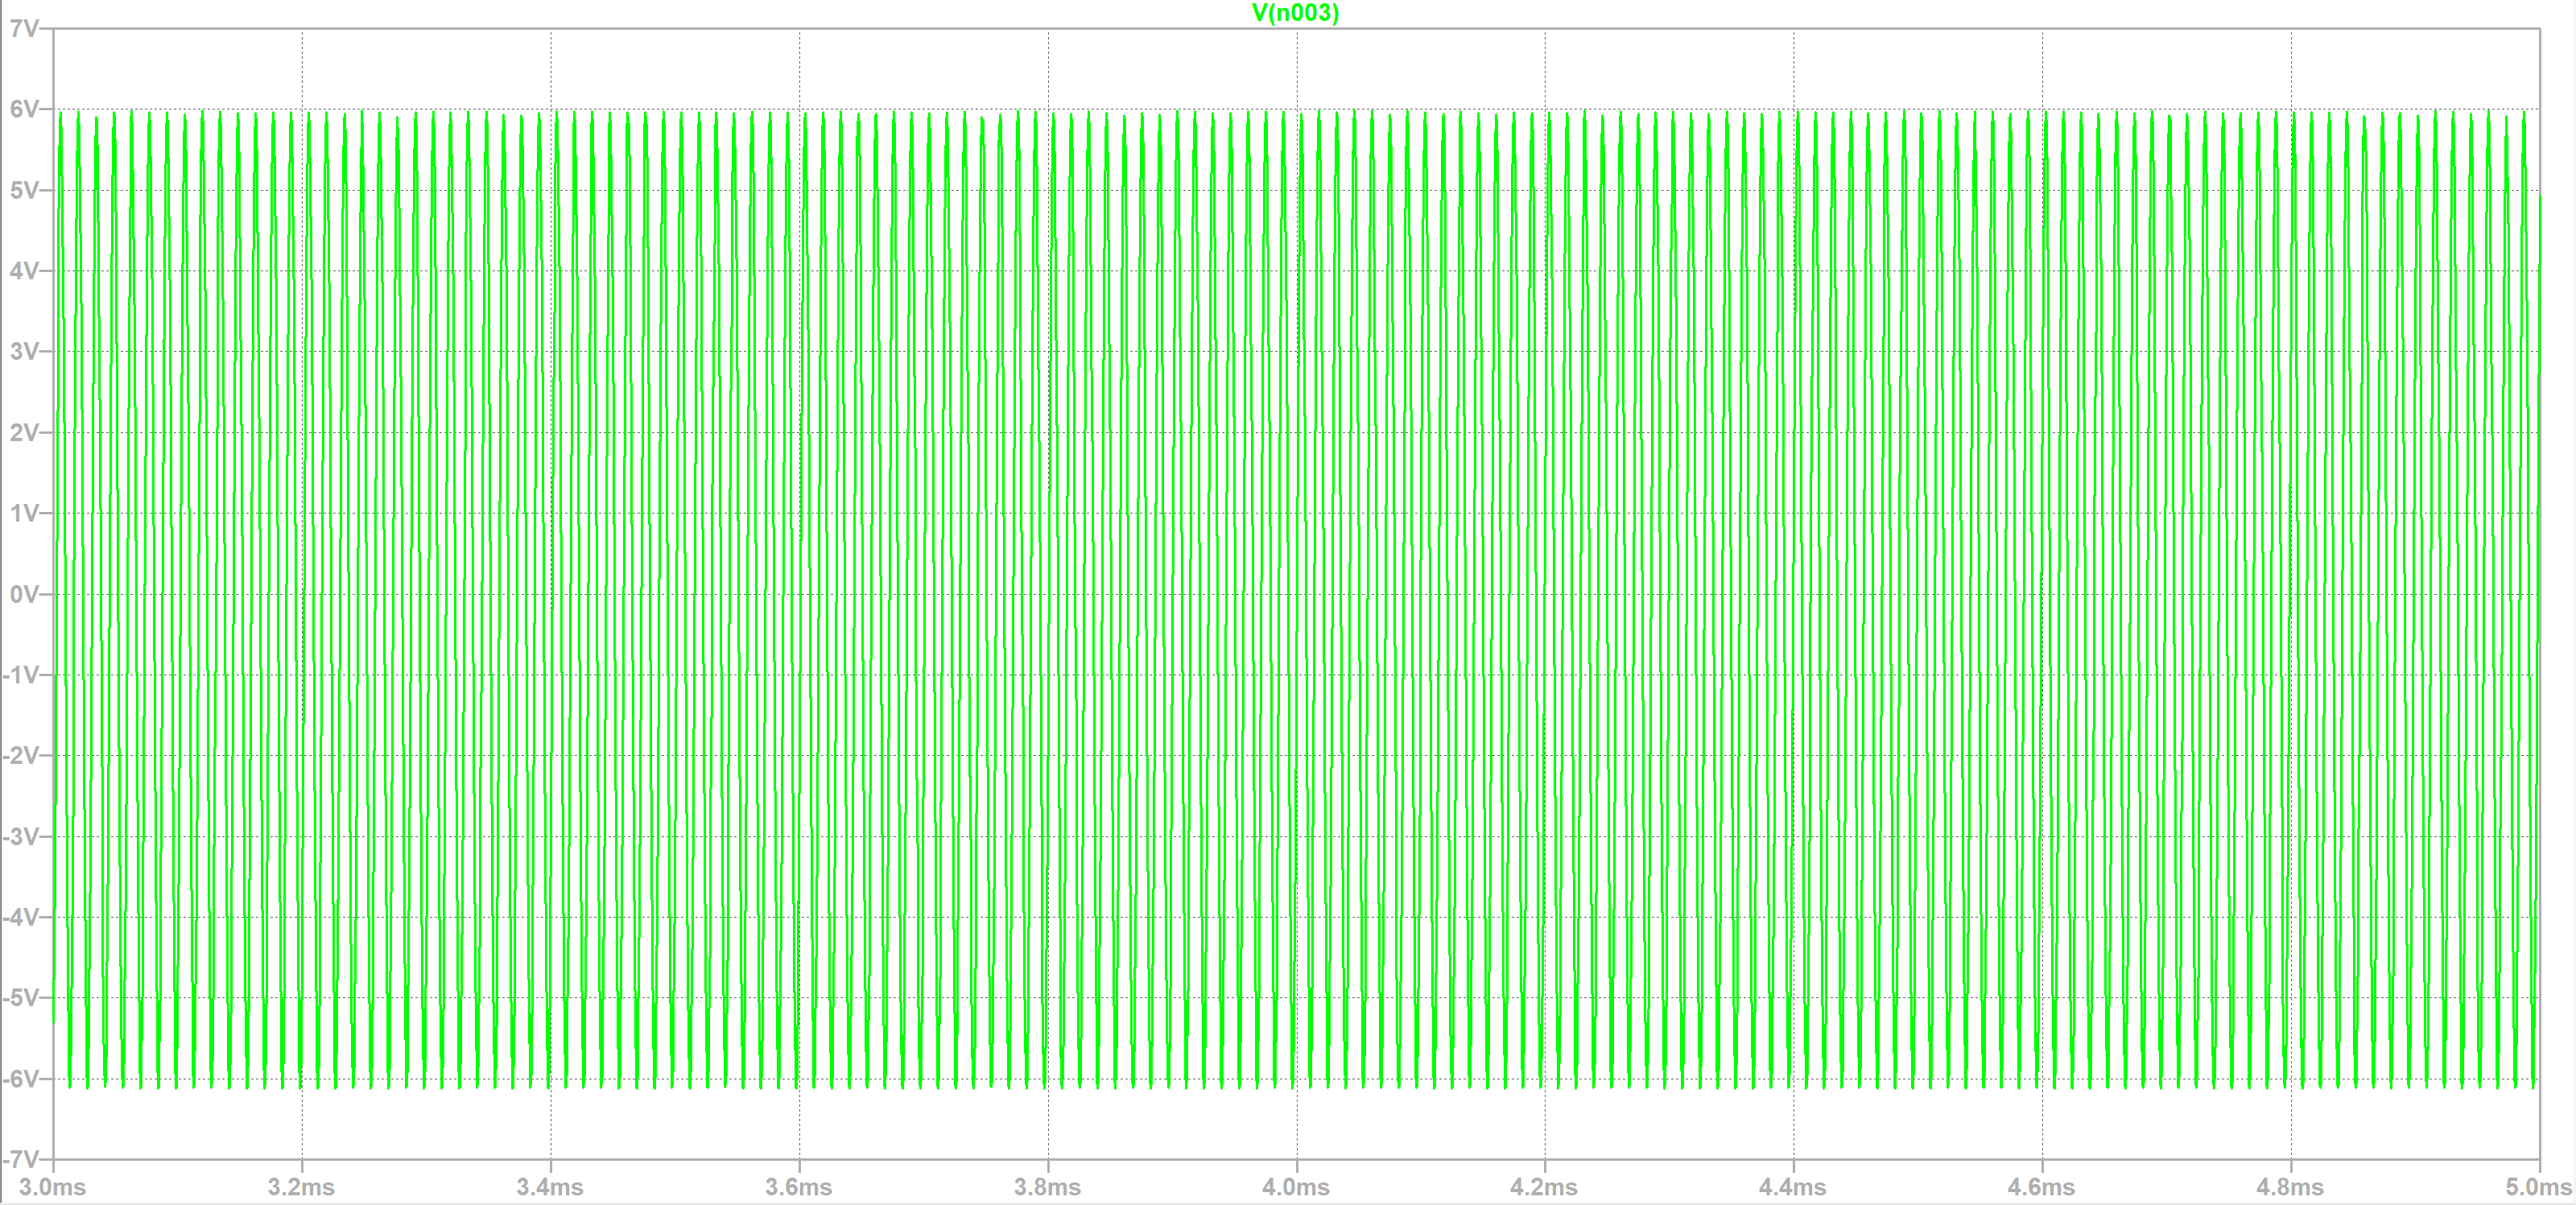
\includegraphics[scale=0.5]{imagenes/variacion_amplitud1.png}
	\caption{Amplitud 6V con R = 0k\ohm}
	\label{fig:ej1_variacion_amplitud}
\end{figure}
\begin{figure}[H]	
	\centering
	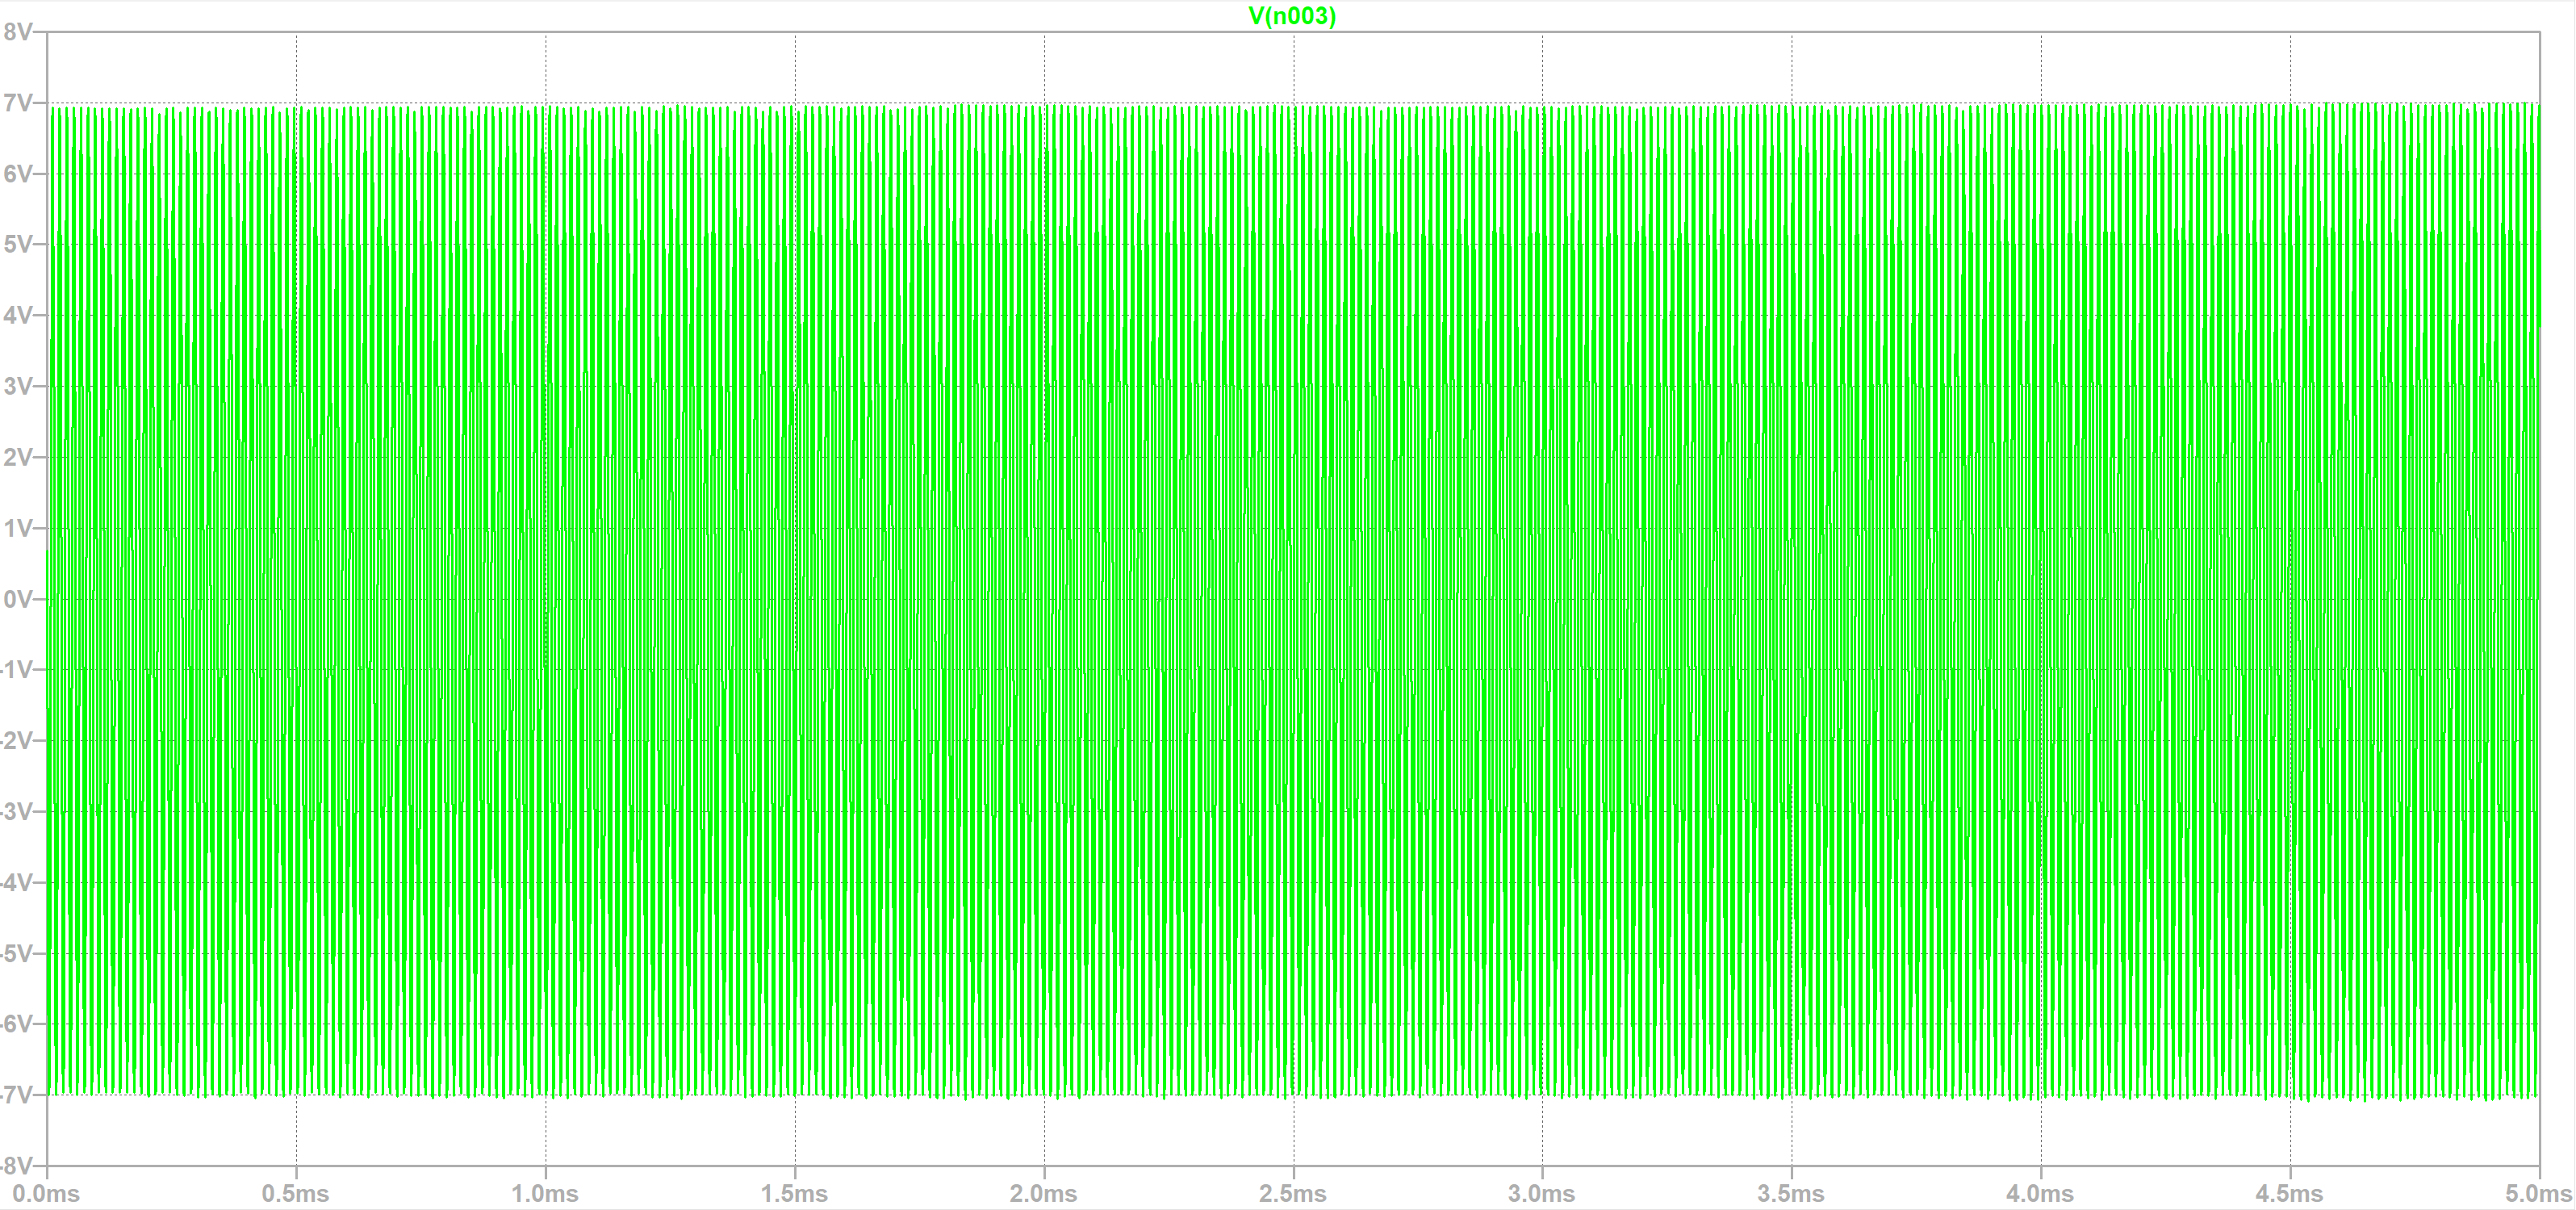
\includegraphics[scale=0.5]{imagenes/variacion_amplitud2.png}
	\caption{Amplitud 7V con R = 50k\ohm}
	\label{fig:ej1_variacion_amplitud}
\end{figure}
También se podría modificar la ganancia del circuito con un no inversor al final, es decir, agregando una etapa de ganancia regulable con un preset.\par
Otra solución consistiría en utilizar diodos de distintas tensiones.

\subsection{Máxima frecuencia de oscilación}

Limitada por el Slew Rate del opamp a elegir, su GBP y la respuesta en frecuencia del transistor.\par
Si bien no hay un máximo teórico para la frecuencia de oscilación, esta está limitada por los factores tecnológicos mencionados anteriormente.\par
A partir de simulaciones se buscó un máximo con los componentes ya elegidos (cuyos valores serán explicitados más adelante en el informe) y se descubrió que no se podía hacer oscilar al circuito a frecuencias mayores a 100kHz, o al menos esperando un tiempo razonable de establecimiento (se fijó el máximo en 1 segundo).

\subsubsection{Análisis de sensibilidades}

$\frac{\partial \beta (s)}{\partial c1} = \frac{\mathrm{c2}\, \mathrm{r2}\, s + 1}{\mathrm{c1}\, \mathrm{r1}\, s + \mathrm{c1}\, \mathrm{r2}\, s + \mathrm{c2}\, \mathrm{r2}\, s + \mathrm{c1}\, \mathrm{c2}\, \mathrm{r1}\, \mathrm{r2}\, s^2 + 1}$\par
$\frac{\partial \beta (s)}{\partial r1} = -\frac{\mathrm{r1}\, \left(\mathrm{c1}\, \mathrm{c2}\, \mathrm{r2}\, s^2 + \mathrm{c1}\, s\right)}{\mathrm{c1}\, \mathrm{c2}\, \mathrm{r1}\, \mathrm{r2}\, s^2 + \left(\mathrm{c1}\, \mathrm{r1} + \mathrm{c1}\, \mathrm{r2} + \mathrm{c2}\, \mathrm{r2}\right)\, s + 1}$\par
$\frac{\partial \beta (s)}{\partial c2} = -\frac{\mathrm{c2}\, \left(\mathrm{c1}\, \mathrm{r1}\, \mathrm{r2}\, s^2 + \mathrm{r2}\, s\right)}{\mathrm{c1}\, \mathrm{c2}\, \mathrm{r1}\, \mathrm{r2}\, s^2 + \left(\mathrm{c1}\, \mathrm{r1} + \mathrm{c1}\, \mathrm{r2} + \mathrm{c2}\, \mathrm{r2}\right)\, s + 1}$\par
$\frac{\partial \beta (s)}{\partial r2} = \frac{\mathrm{c1}\, \mathrm{r1}\, s + 1}{\mathrm{c1}\, \mathrm{r1}\, s + \mathrm{c1}\, \mathrm{r2}\, s + \mathrm{c2}\, \mathrm{r2}\, s + \mathrm{c1}\, \mathrm{c2}\, \mathrm{r1}\, \mathrm{r2}\, s^2 + 1}$\par

Como resultado, se puede observar que el cambio en los componentes resultaría en un corrimiento de la frecuencia de corte del pasabandas, o en la deformación del pasabandas en un pasabajos. El primero cambiaría la frecuencia de oscilación mientras que el segundo agrega otras componentes en frecuencia al oscilador, aumentando su THD. Es por esto que se deberá utilizar un preset de calibración de frecuencia además de que los componentes tendrán que tener la menor tolerancia posible.
\section{Elección de los componentes}

Los componentes a utilizar serán resistencias SMD por las mejores tolerancias de estos componentes y capacitores multicapa por tener una mejor respuesta en frecuencia.

\subsection{OPAMPS}

Se buscó que el GBP sea lo más grande posible para interferir lo menos posible con la frecuencia de oscilación, aunque según el libro de la cátedra, se necesitaría un opamp de $GBP >= 2\cdot \pi\cdot 43\cdot70kHz = 18.91Mhz$ para que este no interfiera, lo cual resulta prácticamente imposible y por eso se busca que interfiera lo menos posible, solucionando la diferencia entre la teoría y la práctica luego con un preset.\par
Se buscó también una alta impedancia de entrada para cumplir idealidades en la realimentación.\par
La impedancia de salida baja también fue tenida en cuenta para no cargar al circuito al que se conecte el generador.\par
Se intentó utilizar un Opamp con THD bajo para así no aumentar el THD simulado.\par
La tensión de alimentación también es importante porque define el rango de valores con el cual podré alimentar al oscilador para que este funcione, consiguiendo así mayor versatilidad a la hora de utilizarlo.\par
Además, se prestó atención al Slew Rate para que no interfiera con la senoidal de oscilación.\par

 	\begin{table}[H] %datos thd simulado
				\centering
 				\begin{tabular}{||c c c c c c c c||} 
 					\hline
					$Opamp$ & Zin & Zout & GBP & Avol & THD & Slew Rate&Vcc\\ [0.5ex] 
 					\hline\hline
					tl082 & $10^{12}\ohm$ & -& 3Mhz& $200\frac{V}{mv}$&<0.0003&$13\frac{V}{\micro s}$&18V\\
					tl072 & $\approx10^{12}\ohm$ & -& 3Mhz& $200\frac{V}{mv}$&<0.0003&$13\frac{V}{\micro s}$&15V\\
 				lm833 & $2^{12}\ohm$ & 37\ohm& 16Mhz& $316\frac{V}{mv}$&<0.0002&$7\frac{V}{\micro s}$&36V\\
					LM741 & $2^6\ohm$ & 75\ohm& 1.5Mhz& $200\frac{V}{mv}$&0.0006&$0.5\frac{V}{\micro s}$&22V\\
					LF353 & $10^{12}\ohm$ &- & 4Mhz& $100\frac{V}{mv}$&<0.0002&$13\frac{V}{\micro s}$&18V\\[1ex] 
					\hline
				\end{tabular}
			\end{table}
			
			Se eligió al TL072 porque ya se había utilizado al TL082 previamente con resultados satisfactorios y no se contaba con este en el pañol. Sin embargo, haciendo un análisis profundo de la tabla se debería haber escogido al LM833 como el opamp a utilizar.
\subsection{Componentes determinantes de la frecuencia de oscilación}

Como se mencionó en la sección \nameref{analsubreal}, la frecuencia de corte del pasabandas de $\beta (s)$ está determinada por $f_0 = \frac{1}{2\cdot \pi \cdot C \cdot R}$. Dado que la frecuencia del oscilador determinada por consigna es de 70kHz, si se fija a C = 1nF, la resistencia R deberá valer teóricamente 2273 \ohm para el correcto funcionamiento del circuito. Sin embargo, por los problemas mencionados anteriormente producidos por el GBP limitado del opamp, se elige utilizar una resistencia de $R_2 = 2.2k$ y un preset en donde se sitúa la resistencia $R_1$ en el circuito. Este preset se pretende que pueda variar entre 2k\ohm y 3k\ohm  con suficiente precisión como para ajustar correctamente la frecuencia, por lo que se eligió un preset de 5k\ohm para cubrir todos los casos. 

\subsection{Componentes para el CAG}

El transistor MPF102, el diodo 1N4148 y el diodo Zener 1N5230 están determinados por consigna. Sin embargo, en pañol no se contaba con el diodo Zener requerido, por lo que se utilizó el diodo DZ4V7-05 que sí brindaba el pañol. Este último es un diodo Zener de 4.7V. \par

Como el diodo Zener junto al común determinarán la tensión a la cual se activará el control de ganancia, con el transistor funcionando como resistencia. Es por esto que se espera que el control se active en una tensión cercana a los 5.4 V y que la onda sinusoidal resultante del oscilador por ende tendrá una tensión pico algo superior a 5.5V.\par

Para decidir los valores de las resistencias, se pide que la variación en la relación $\frac{R_3}{R_4}$ sea simétrica con respecto a 2 para las oscilaciones de la tensión en el gate del transistor. Esto se pide así para que la relación converja a 2 luego de un cierto tiempo de establecimiento. Observando las curvas de resistencia para el transistor, se aprecia una resistencia de 0.54k\ohm para una tensión de gate de 0.5V. Como se sabe que recién conectado el circuito se apreciará la oscilación más grande de todas y el transistor por ende tendrá su valor más alto de resistencia, se utiliza este valor para las cuentas iniciales que determinarán los -valores de $R_3$ y $R_4$.\par

Se plantea entonces el siguiente sistema de ecuaciones, teniendo en cuenta una variación simétrica de 0.1V y llamando a la resistencia agregada del transistor $R_t$:
	 \begin{equation}
  	   \left\{
	  	    \begin{array}{ll}
		 					\frac{R_3}{R_4} = 2.1     \\
			 				\frac{R_3}{R_4+R_t} = 1.9\\
	     	 \end{array}
	     	\right.
 	\end{equation}
 	Entonces, usando $R_t= 0.54k\ohm$,  llegamos a $R_4 = 51.3k\ohm$ y a $R_3 = 107.73k\ohm$. Estos valores luego serán modificados al simular, pero se espera que se acerquen a los teóricos calculados de la manera predicha anteriormente.\par 
Luego de la simulación se llega a la conclusión que $R_4 = 51k\ohm$ y $R_3 = 106k\ohm$, que será implementada mediante una combinación serie de resistencias.
Como se dijo en la sección \nameref{cag}, el capacitor en paralelo con la resistencia del CAG son componentes clave para determinar el correcto funcionamiento del CAG al necesitar que el tiempo en que se descargue el capacitor sea lo suficientemente lento como para que el capacitor se cargue y se descargue en un ciclo de onda, manteniéndose constante la mayor parte del tiempo para lograr así mantener durante ese período a la resistencia del transistor en el valor de convergencia, y así se busca que el factor de tiempo RC sea grande. Se determina por lo tanto que $R_x = 1M\ohm$ y $C_3 = 1\micro F$.
El diagrama de polos y ceros teórico con la resistencia del transistor nula es:\par

\begin{figure}[H]	
	\centering
	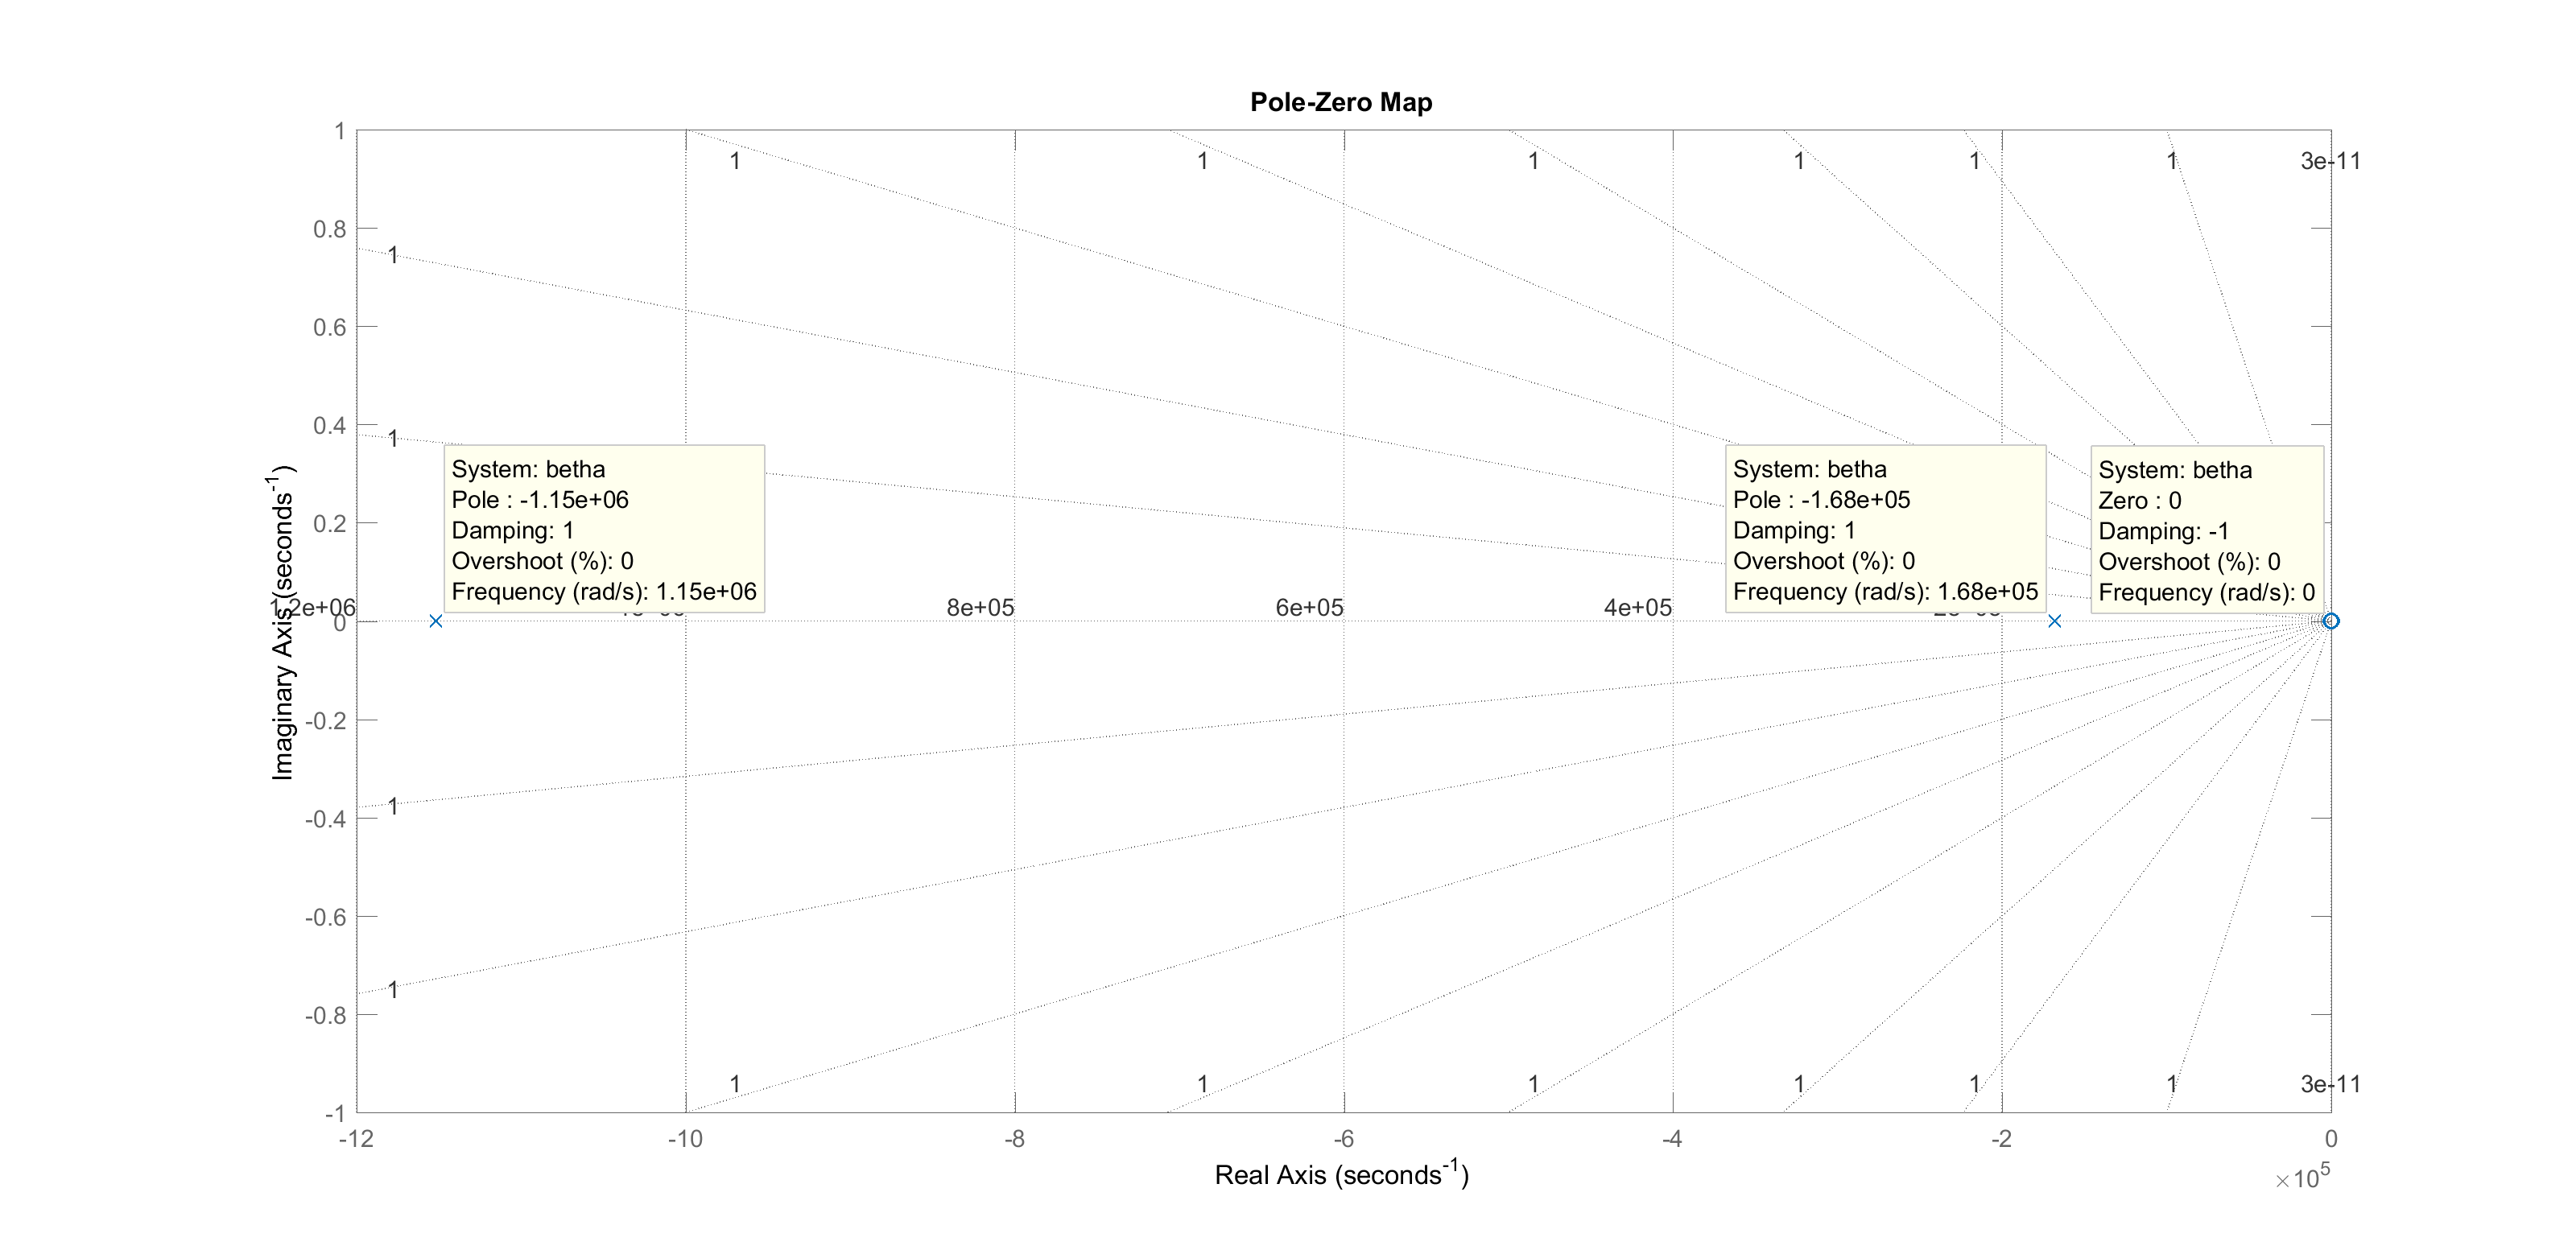
\includegraphics[scale=0.2]{imagenes/polos_ceros_betha.png}
	\caption{Polos y ceros para la ganancia de lazo abierto para resistencia nula del transistor}
	\label{fig:ej1_polos_ceros_betha}
\end{figure}

\begin{figure}[H]	
	\centering
	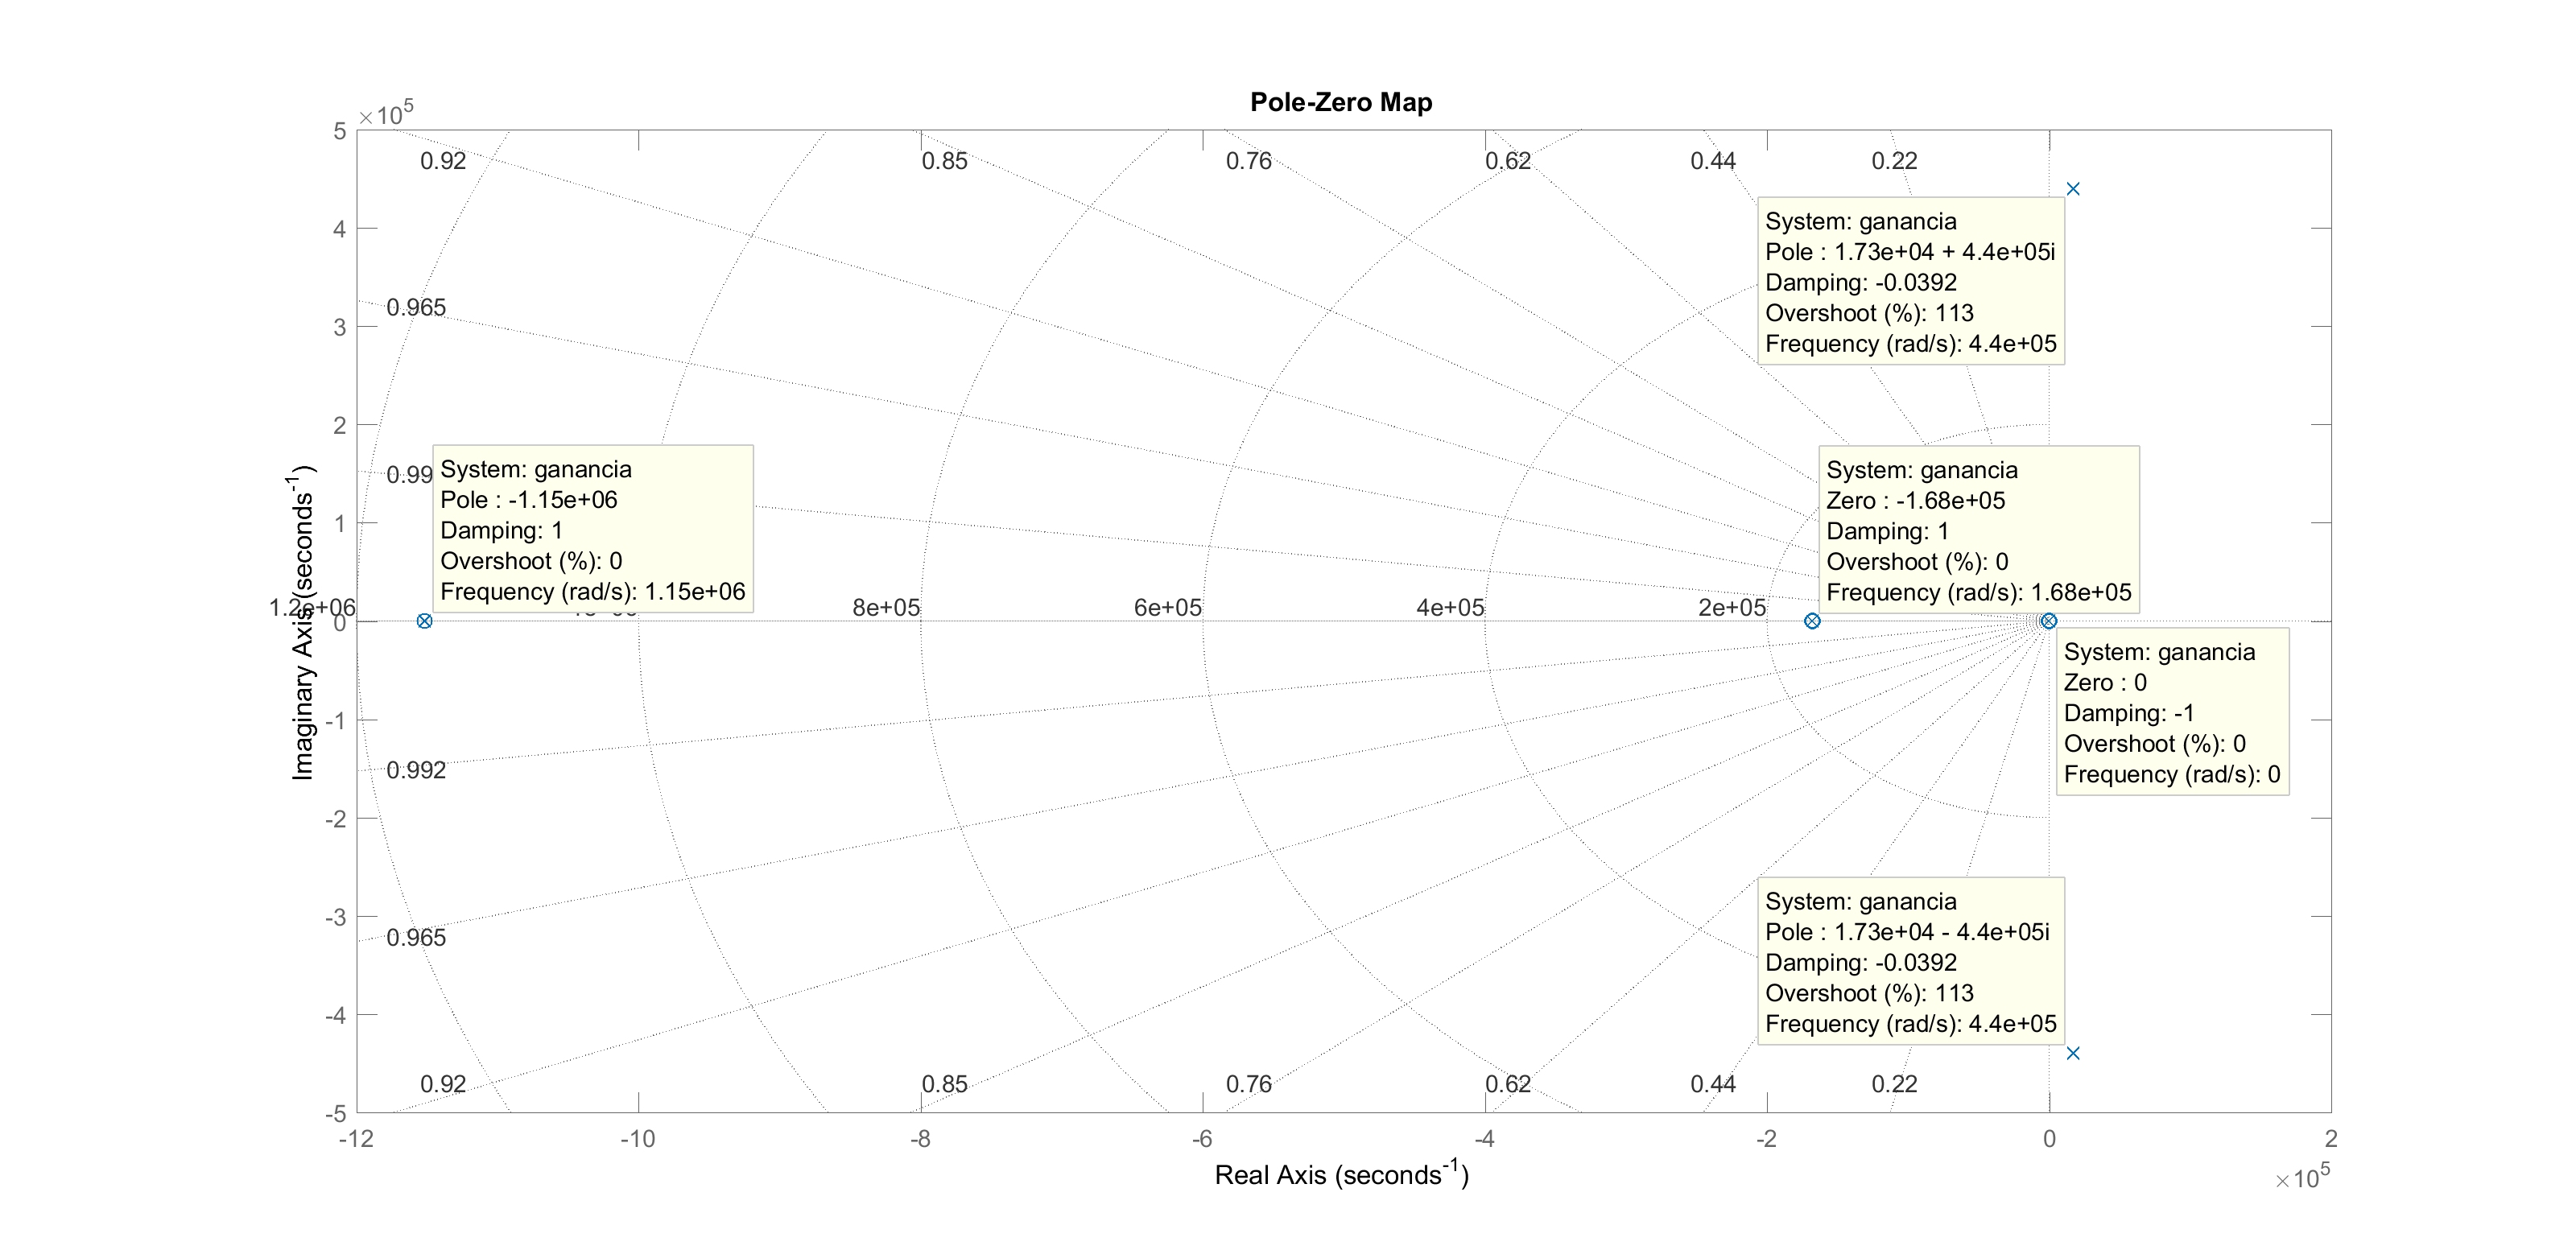
\includegraphics[scale=0.2]{imagenes/polos_ceros_T.png}
	\caption{Polos y ceros para la ganancia completa del sistema, lazo cerrado.}
	\label{fig:ej1_polos_ceros_T}
\end{figure}

Se muestra el diagrama de polos y ceros para cuando el transistor llega a su valor final de resistencia, es decir, cuando el circuito oscila. Deben notarse las singularidades en el eje imaginario.

\begin{figure}[H]	
	\centering
	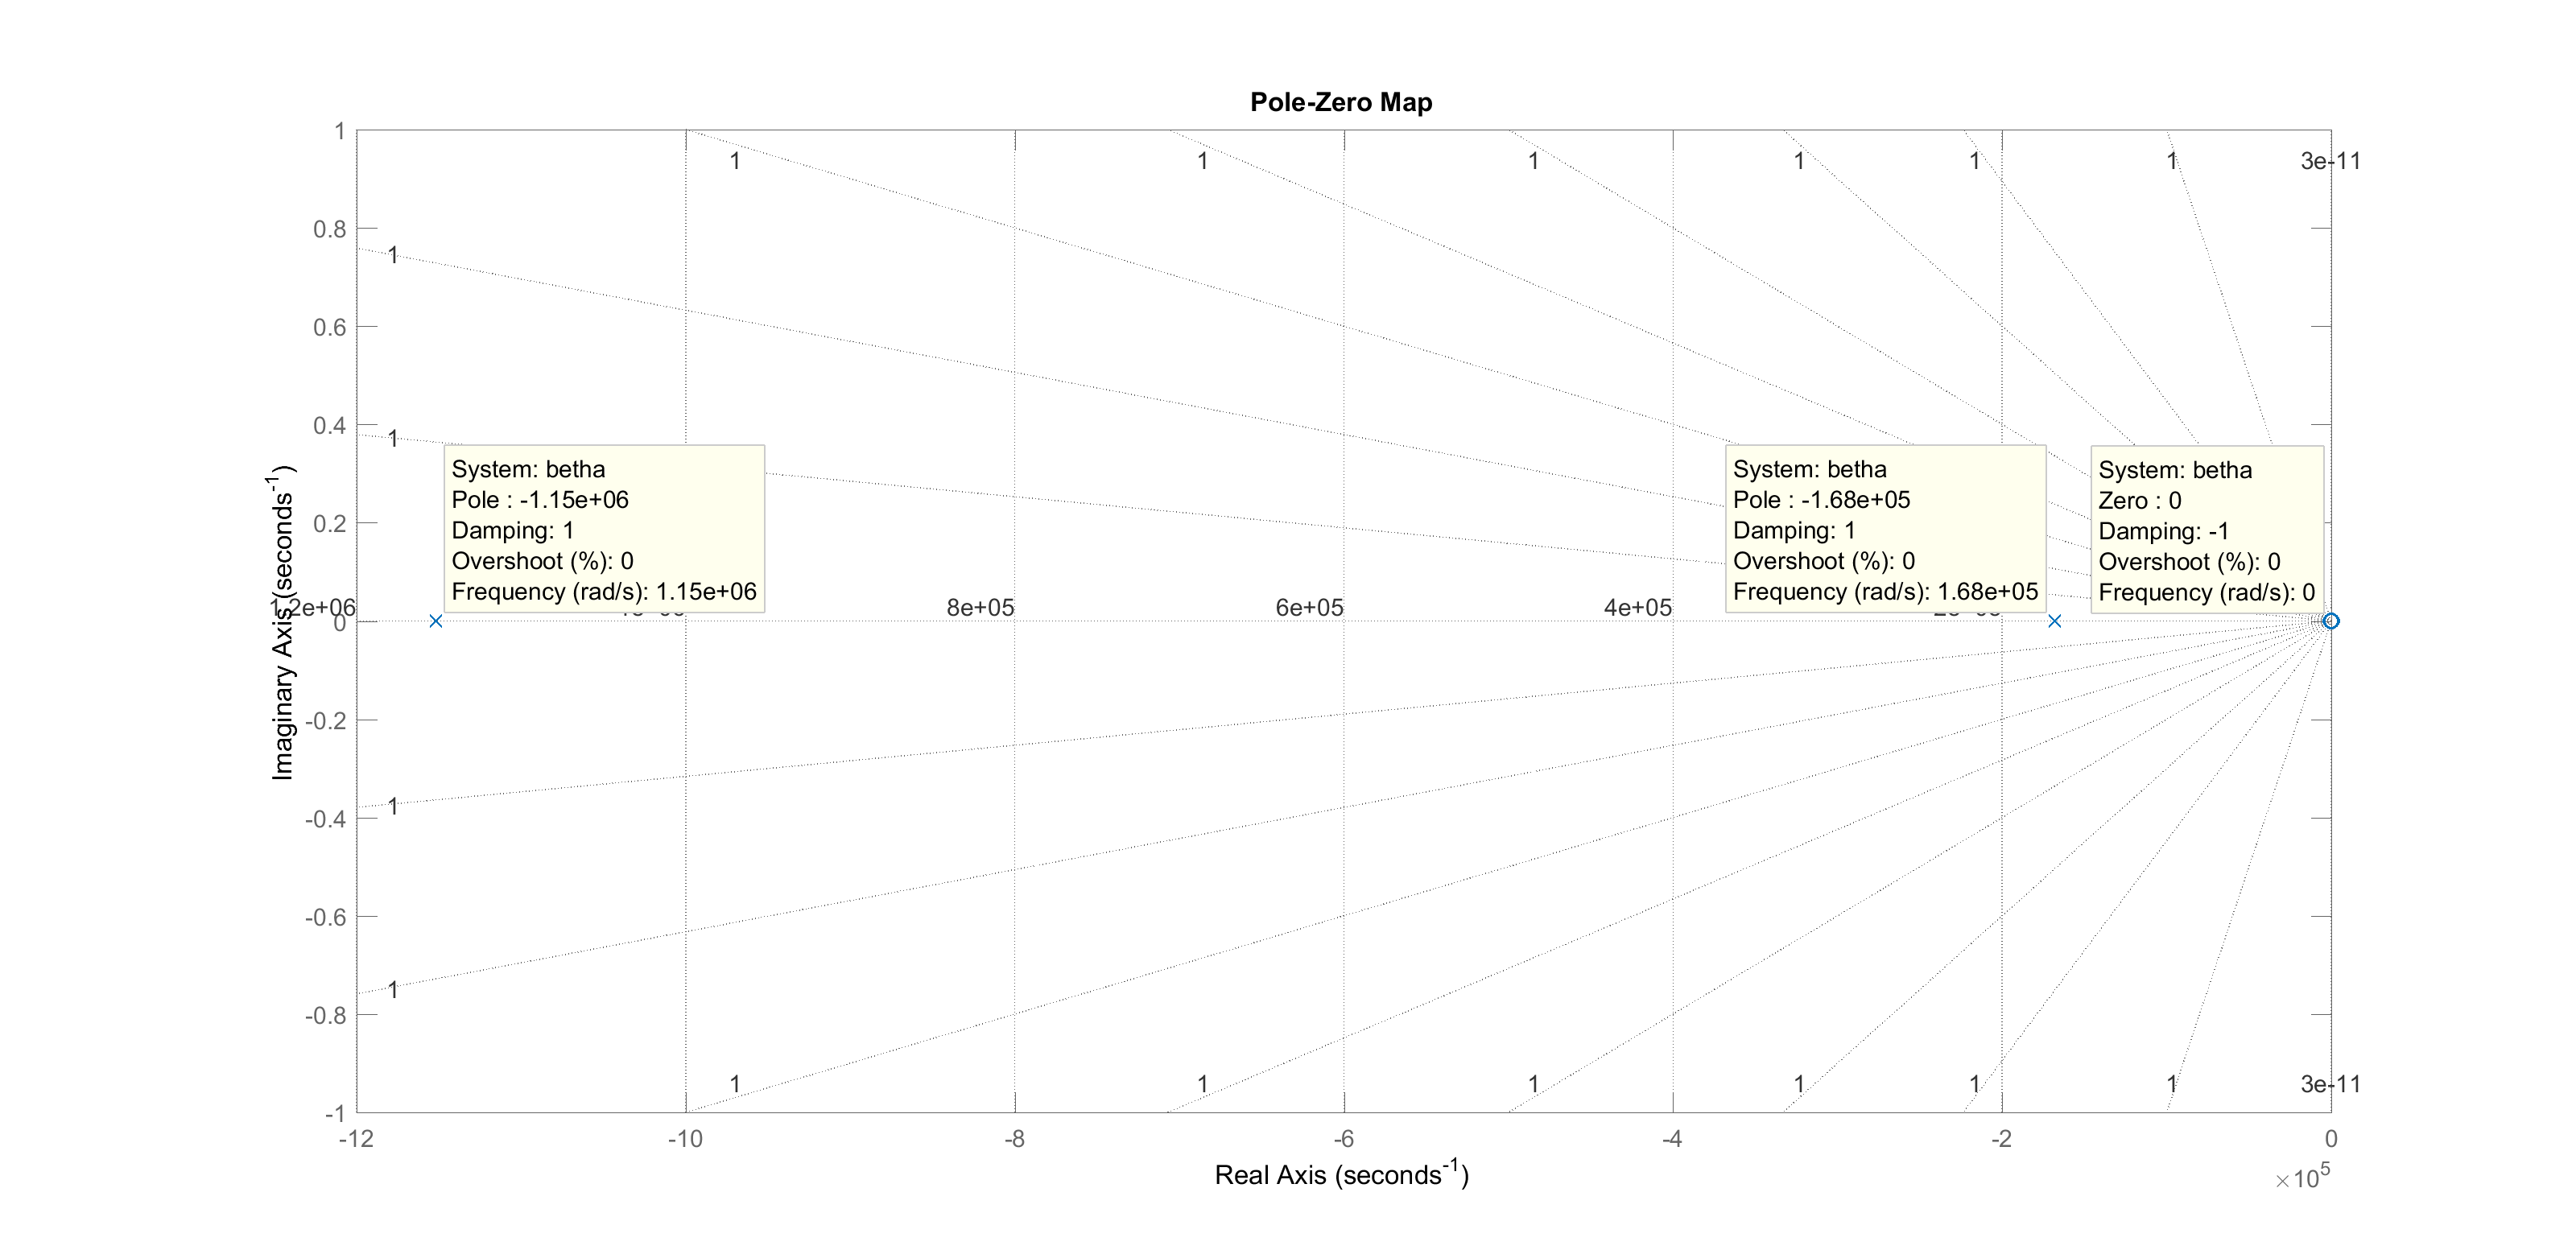
\includegraphics[scale=0.2]{imagenes/polos_ceros_betha_rfinal.png}
	\caption{Polos y ceros para la ganancia de lazo abierto. Resistencia del transistor ya establecida, cumpliendo BarkHausen.}
	\label{fig:ej1_polos_ceros_ganancia_rfinal}
\end{figure}

\begin{figure}[H]	
	\centering
	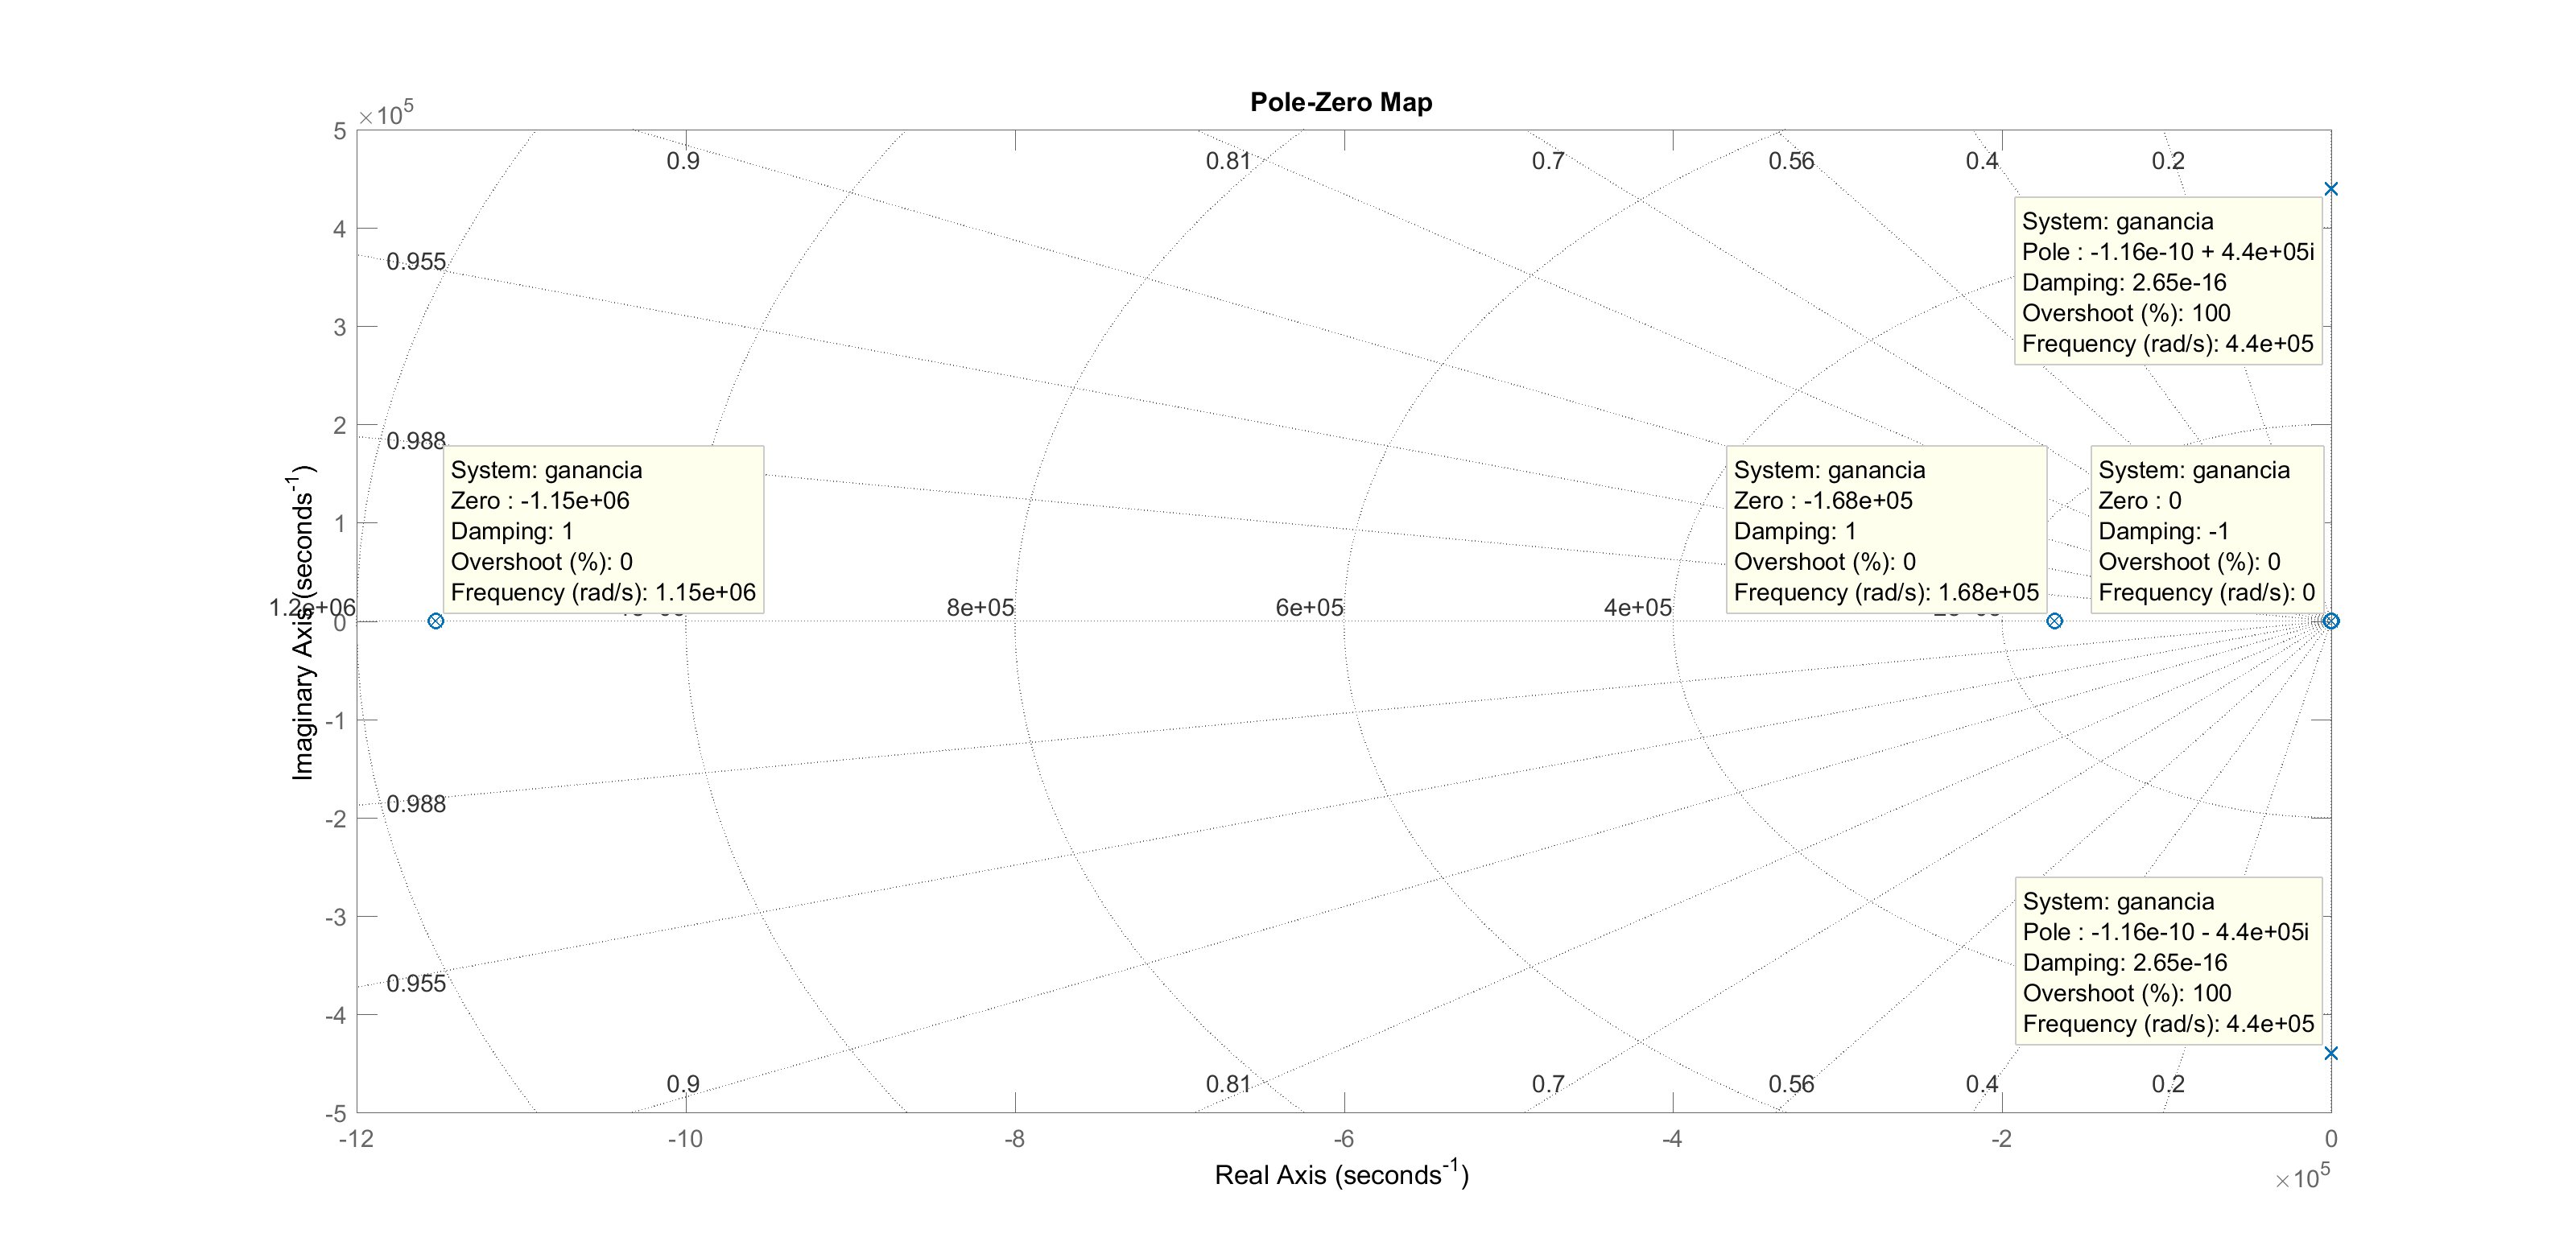
\includegraphics[scale=0.2]{imagenes/polos_ceros_ganancia_rfinal.png}
	\caption{Polos y ceros para la ganancia completa del sistema. Resistencia del transistor ya establecida, cumpliendo BarkHausen.}
	\label{fig:ej1_polos_ceros_ganancia_rfinal}
\end{figure}

\section{Simulación}

\subsection{Distorsión Armónica}

El oscilador no dará señales senoidales completamente puras o ideales. Esto quiere decir que la señal resultante no tendrá componentes en una única frecuencia (la de oscilación, 70kHz) sino que habrá potencia perdida en otras frecuencias. Esta pérdida de potencia estará distribuída principalmente en los armónicos de la frecuencia fundamental. Es por esto que una medida bastante fiel de qué tan ''bueno'' es un oscilador es el THD (Total Harmonic Distortion), que compara la potencia del armónico fundamental contra la potencia total del oscilador bajo la fórmula $THD = \frac{P_{armonicos}}{P_{total}}$, donde $P_{total}$ es la suma de las potencias de todos los armónicos incluyendo a la frecuencia de oscilación y $P_{armonicos}$ es la potencia de todos los armónicos menos la de la frecuencia de oscilación.\par
Así, al multiplicar por 100 al THD, este da un porcentaje de pérdida de potencia en frecuencias que no son de interés.\par
Se utilizó el LTSPICE para simular la distorsión armónica del circuito propuesto con los valores de los componentes ya fijados. 

\begin{figure}[H]	
	\centering
	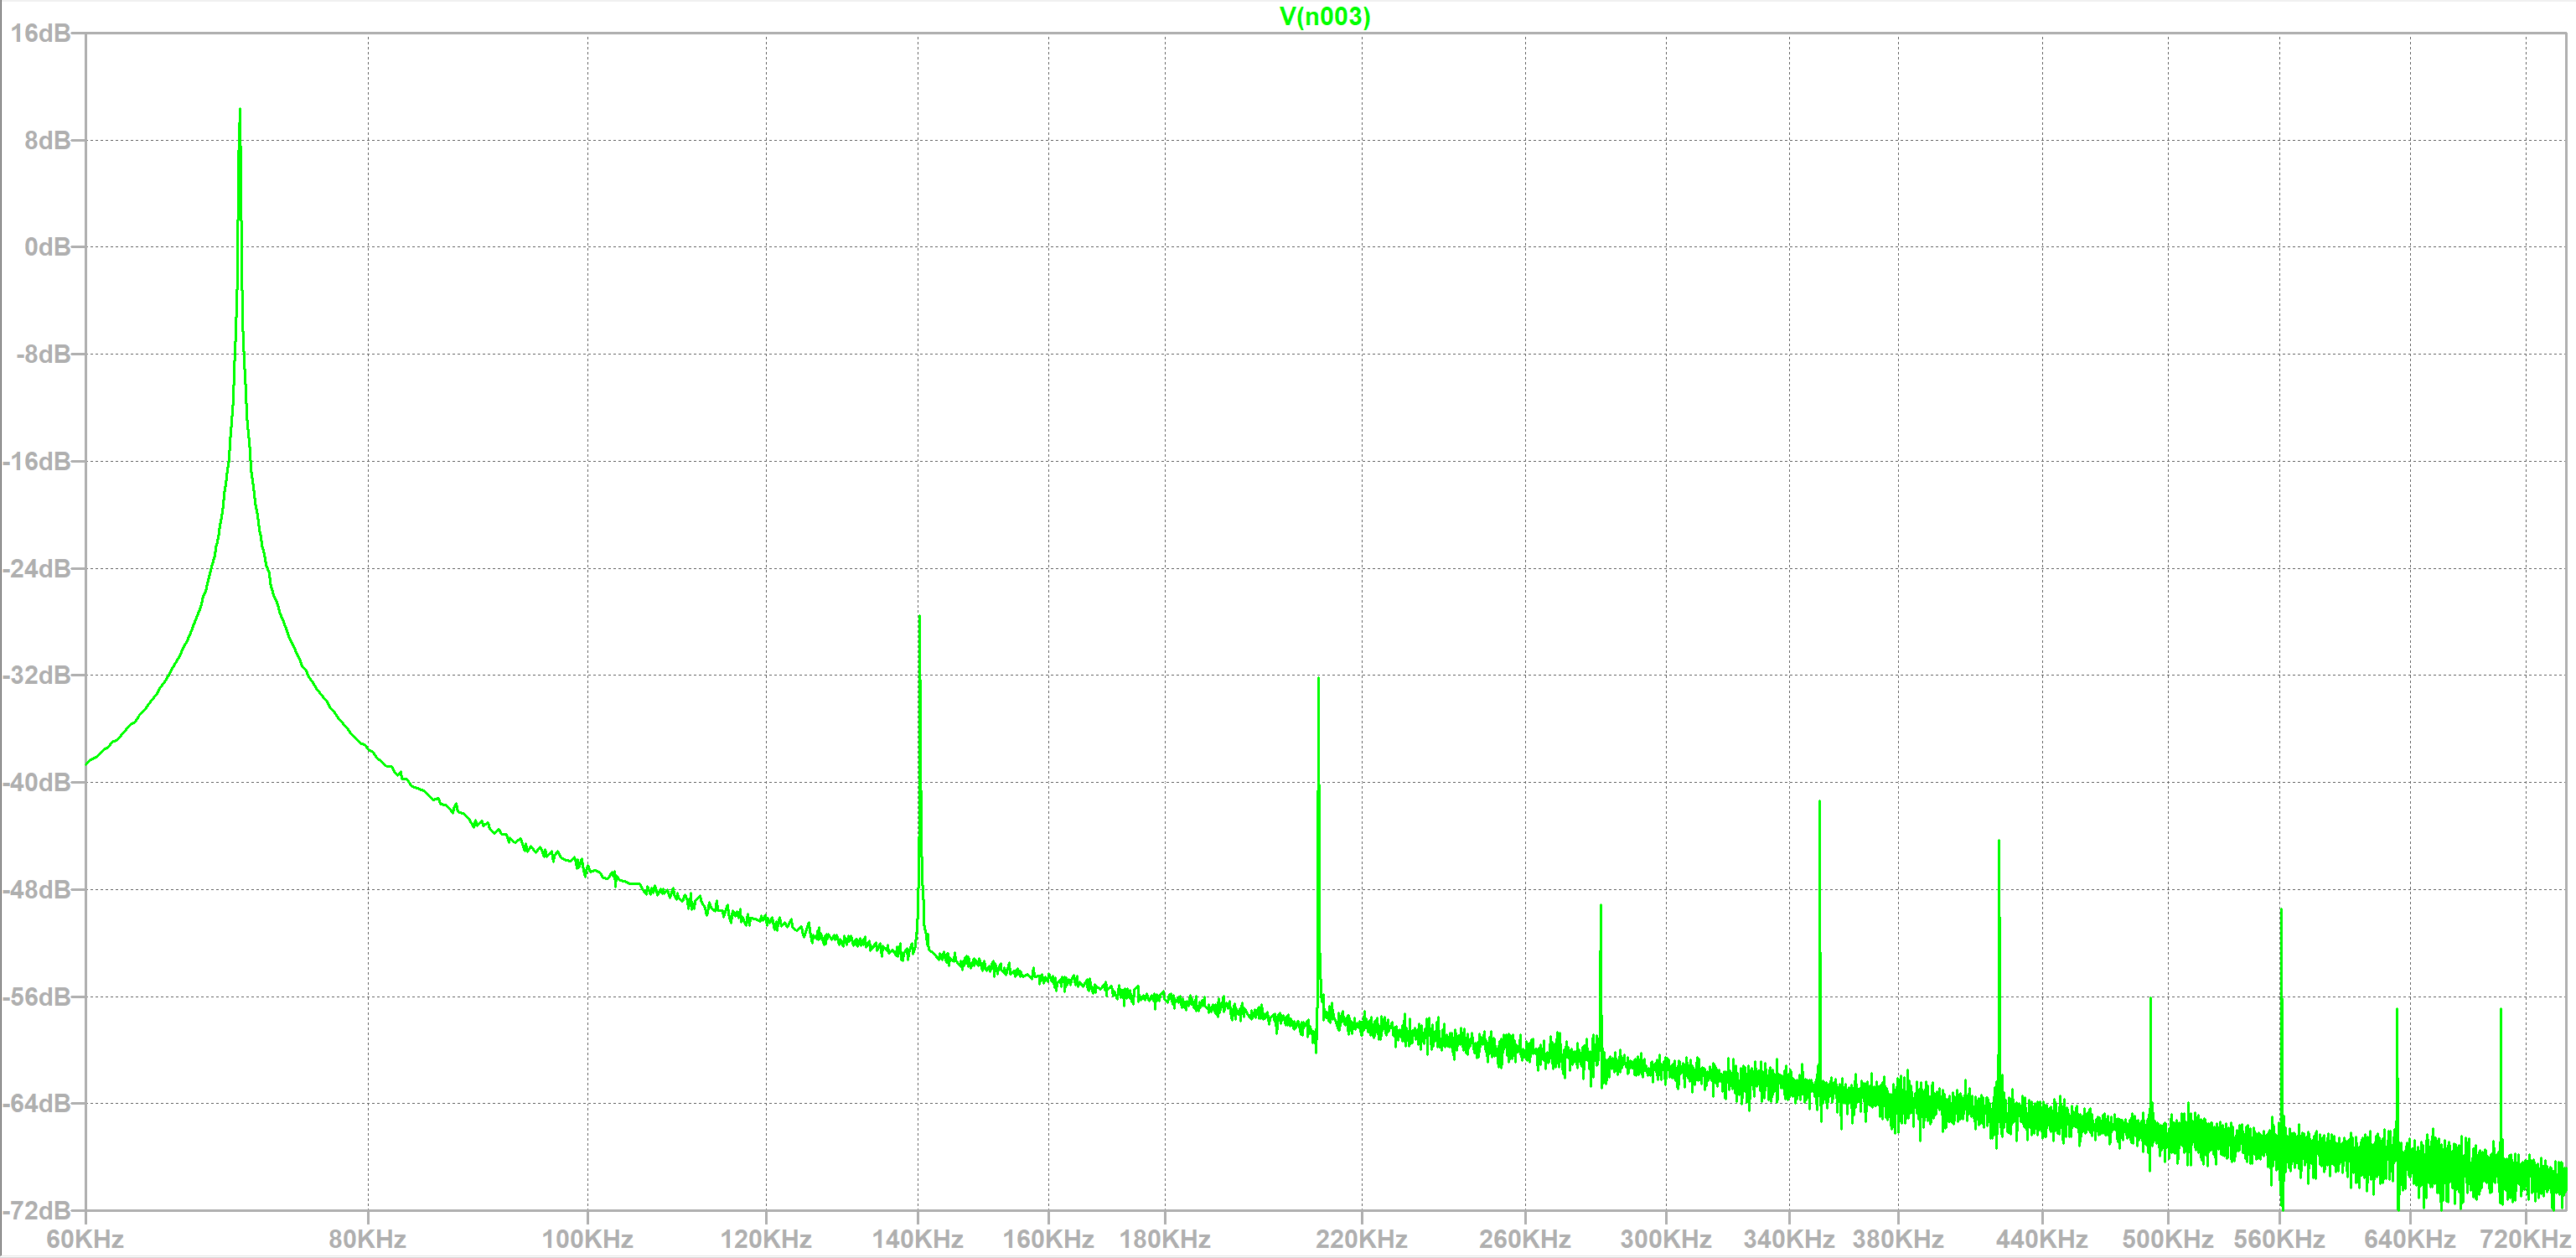
\includegraphics[scale=0.5]{imagenes/thd_simulado.png}
	\caption{FFT en LTSPICE del oscilador armado}
	\label{fig:ej1_thd_simulado}
\end{figure}

De este gráfico, con el cursor, se obtuvo la siguiente tabla de datos: 

	\begin{table}[H] %datos thd simulado
				\centering
 				\begin{tabular}{||c c||} 
 					\hline
					$frecuencia(kHz)$ & Potencia(dB)\\ [0.5ex] 
 					\hline\hline
					70.2 & $10.03$\\
					140.3 & $-28.15$\\
					210.5 & $-32.5$\\
					280.6 & $-49.17$\\
					350.8 & $-41.5$\\
					420 & $-44.33$\\
					491.1 & $-56,06$\\
					561,5 & $-49,5$\\
					631.45 & $-56.89$\\
					701.59 & $-57.09$\\[1ex] 
					\hline
				\end{tabular}
			\end{table}
Usando la fórmula previamente mencionada para medir el THD, se consiguió un\par
\begin{center}
$THD_{simulado} = 0.027$
\end{center}

\subsection{Tensiones de alimentación}

Si Vcc es la tensión con la que se alimenta al opamp, se requiere una tensión de alimentación que no sature a la hora de generar la señal. Es por esto que se requiere Vcc supere con un margen lo suficientemente grande a la tensión pico del generador. Es así como se decide que Vcc estará entre los valores 7V y 15V para el correcto funcionamiento del oscilador.
\subsection{Tensión y resistencias del transistor en estacionario}

Dados los valores de resistencias elegidos, como se espera que la relación $\frac{R_3}{R_4+R_{tFinal}}=2$ luego de acabado un cierto tiempo de establecimiento, entonces como $R_3 =  106k\ohm$ y $R_4 =  51k\ohm$, $R_{tFinal} = 2k\ohm$. Esto se puede observar en la simulación: 

\begin{figure}[H]	
	\centering
	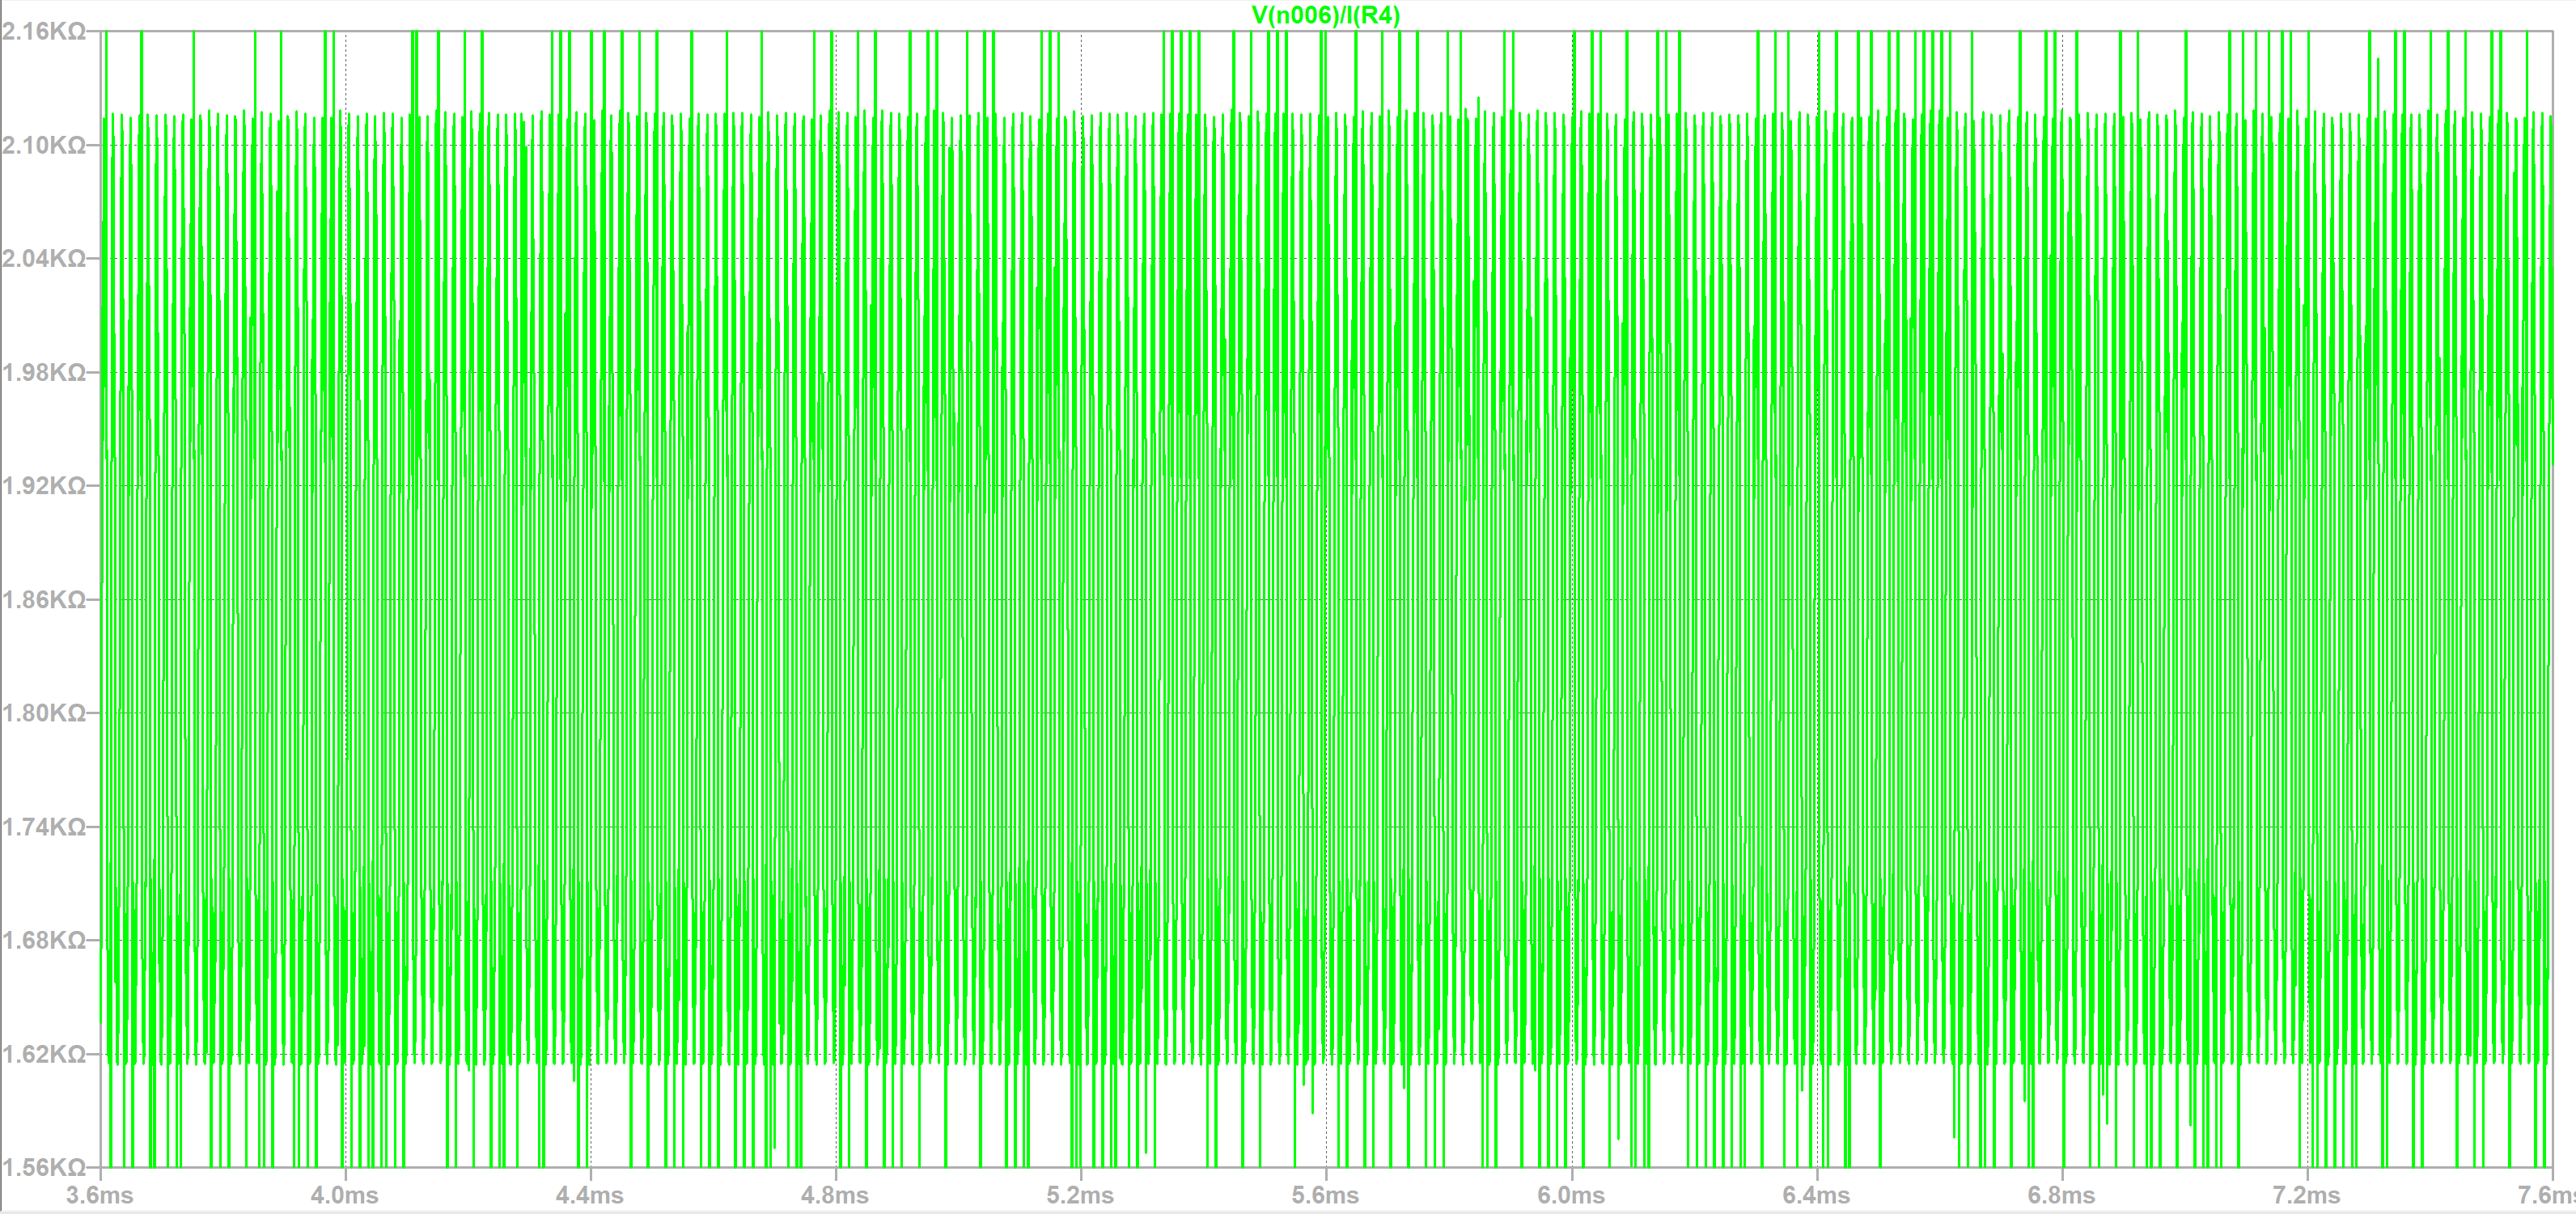
\includegraphics[scale=0.5]{imagenes/resistencia_trans_simulada.png}
	\caption{Resistencia del transistor en estacionario}
	\label{fig:ej1_resistencia_trans_simulada}
\end{figure}

donde los valores de resistencia oscilan alrededor de los 2k\ohm.\par

Además, al fijar el valor de resistencia del transistor también se tiene que fijar el valor de tensión del GATE, por lo que se espera que oscile poco entre un valor fijo. Para determinar el valor se observan las curvas simuladas, en la subsección \nameref{curvas_trans} y se recuerda que pedimos dos condiciones para que se pueda considerar a la curva como aquella representativa en estado estacionario:
\begin{enumerate}
\item La tensión Vds no podrá superar los 0.1V y aún así deberá llegar el transistor a la resistencia de 2k\ohm necesaria en tiempo estacionario. Esto es así porque a partir de los 0.1V comienza el comportamiento no lineal para el transistor.
\item El cambio de resistencia no tendrá que ser abrupto con respecto a la tensión Vds, porque eso implicaría comportamiento erráticos en la tensión y en la corriente que podría alterar al oscilador. 
\end{enumerate}
Vemos de aquí que las dos curvas que cumplen con estas condiciones son las de Vgs =-3.1V y -3.2V,  por lo que se descubre que el valor de oscilación para la tensión de GATE estará entonces centrado en algún valor en el medio de estos dos, cercano a -3.15V.\par
Se confirma esta teoría con la simulación:

\begin{figure}[H]	
	\centering
	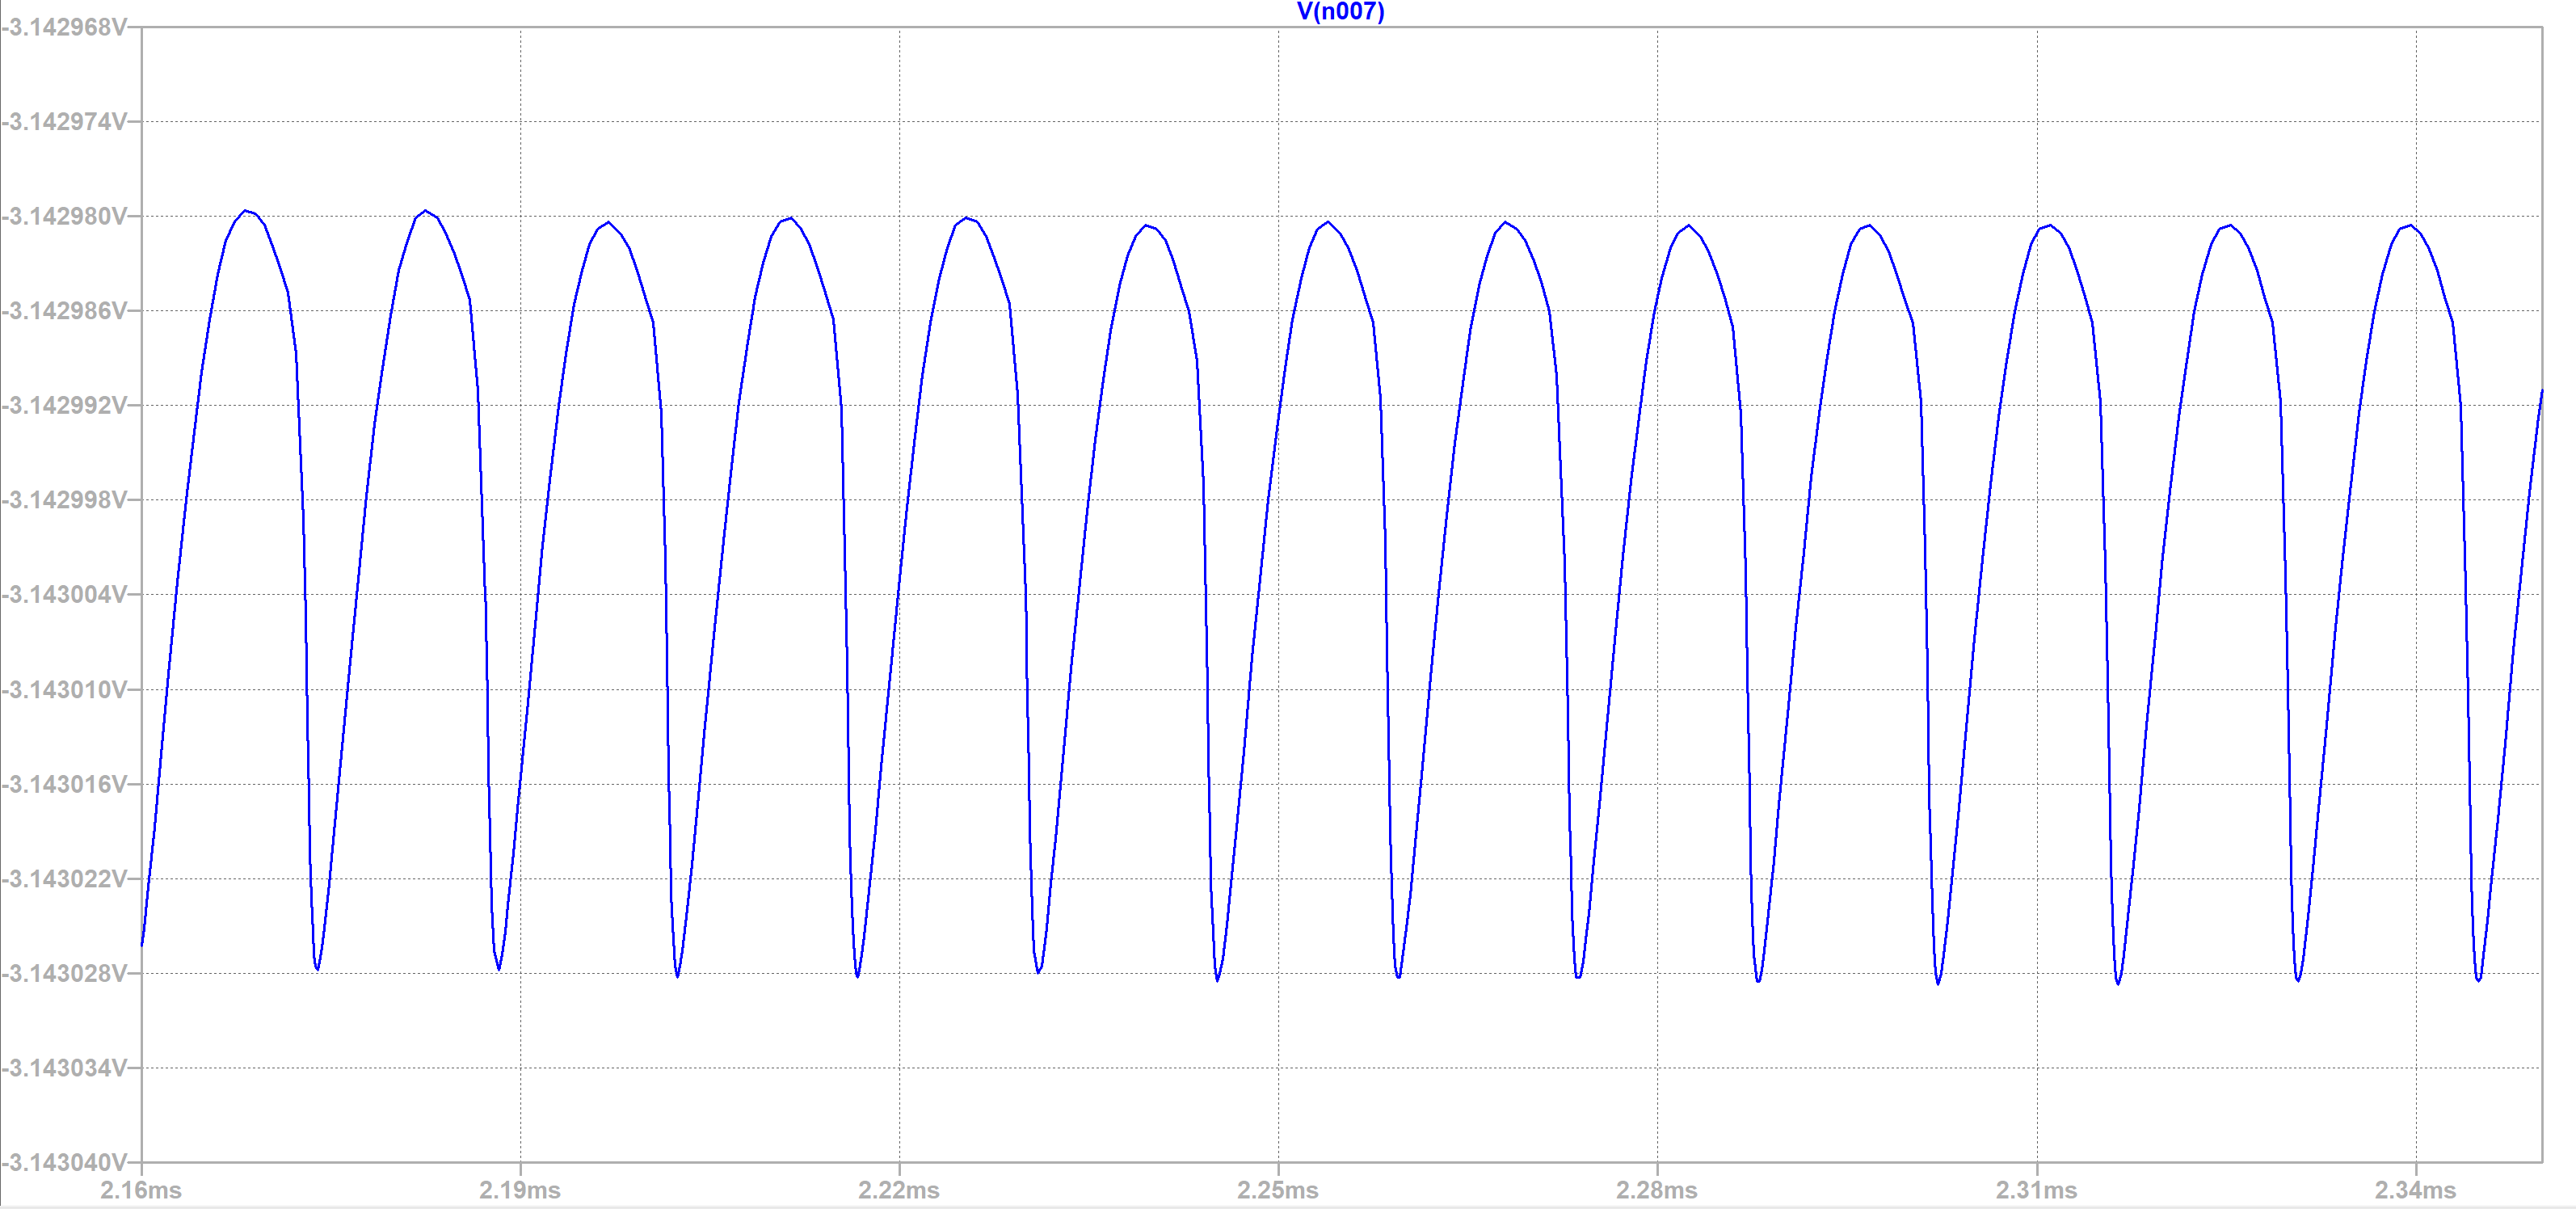
\includegraphics[scale=0.5]{imagenes/oscilaciones_vgs.png}
	\caption{Valor central para VGS en estado estacionario}
	\label{fig:ej1_oscilaciones_vgs}
\end{figure}

\section{Mediciones}

\subsection{Respuesta en tiempo}
La oscilación resultante observada en el osciloscopio, con los presets ya ajustados fue:
\begin{figure}[H]	
	\centering
	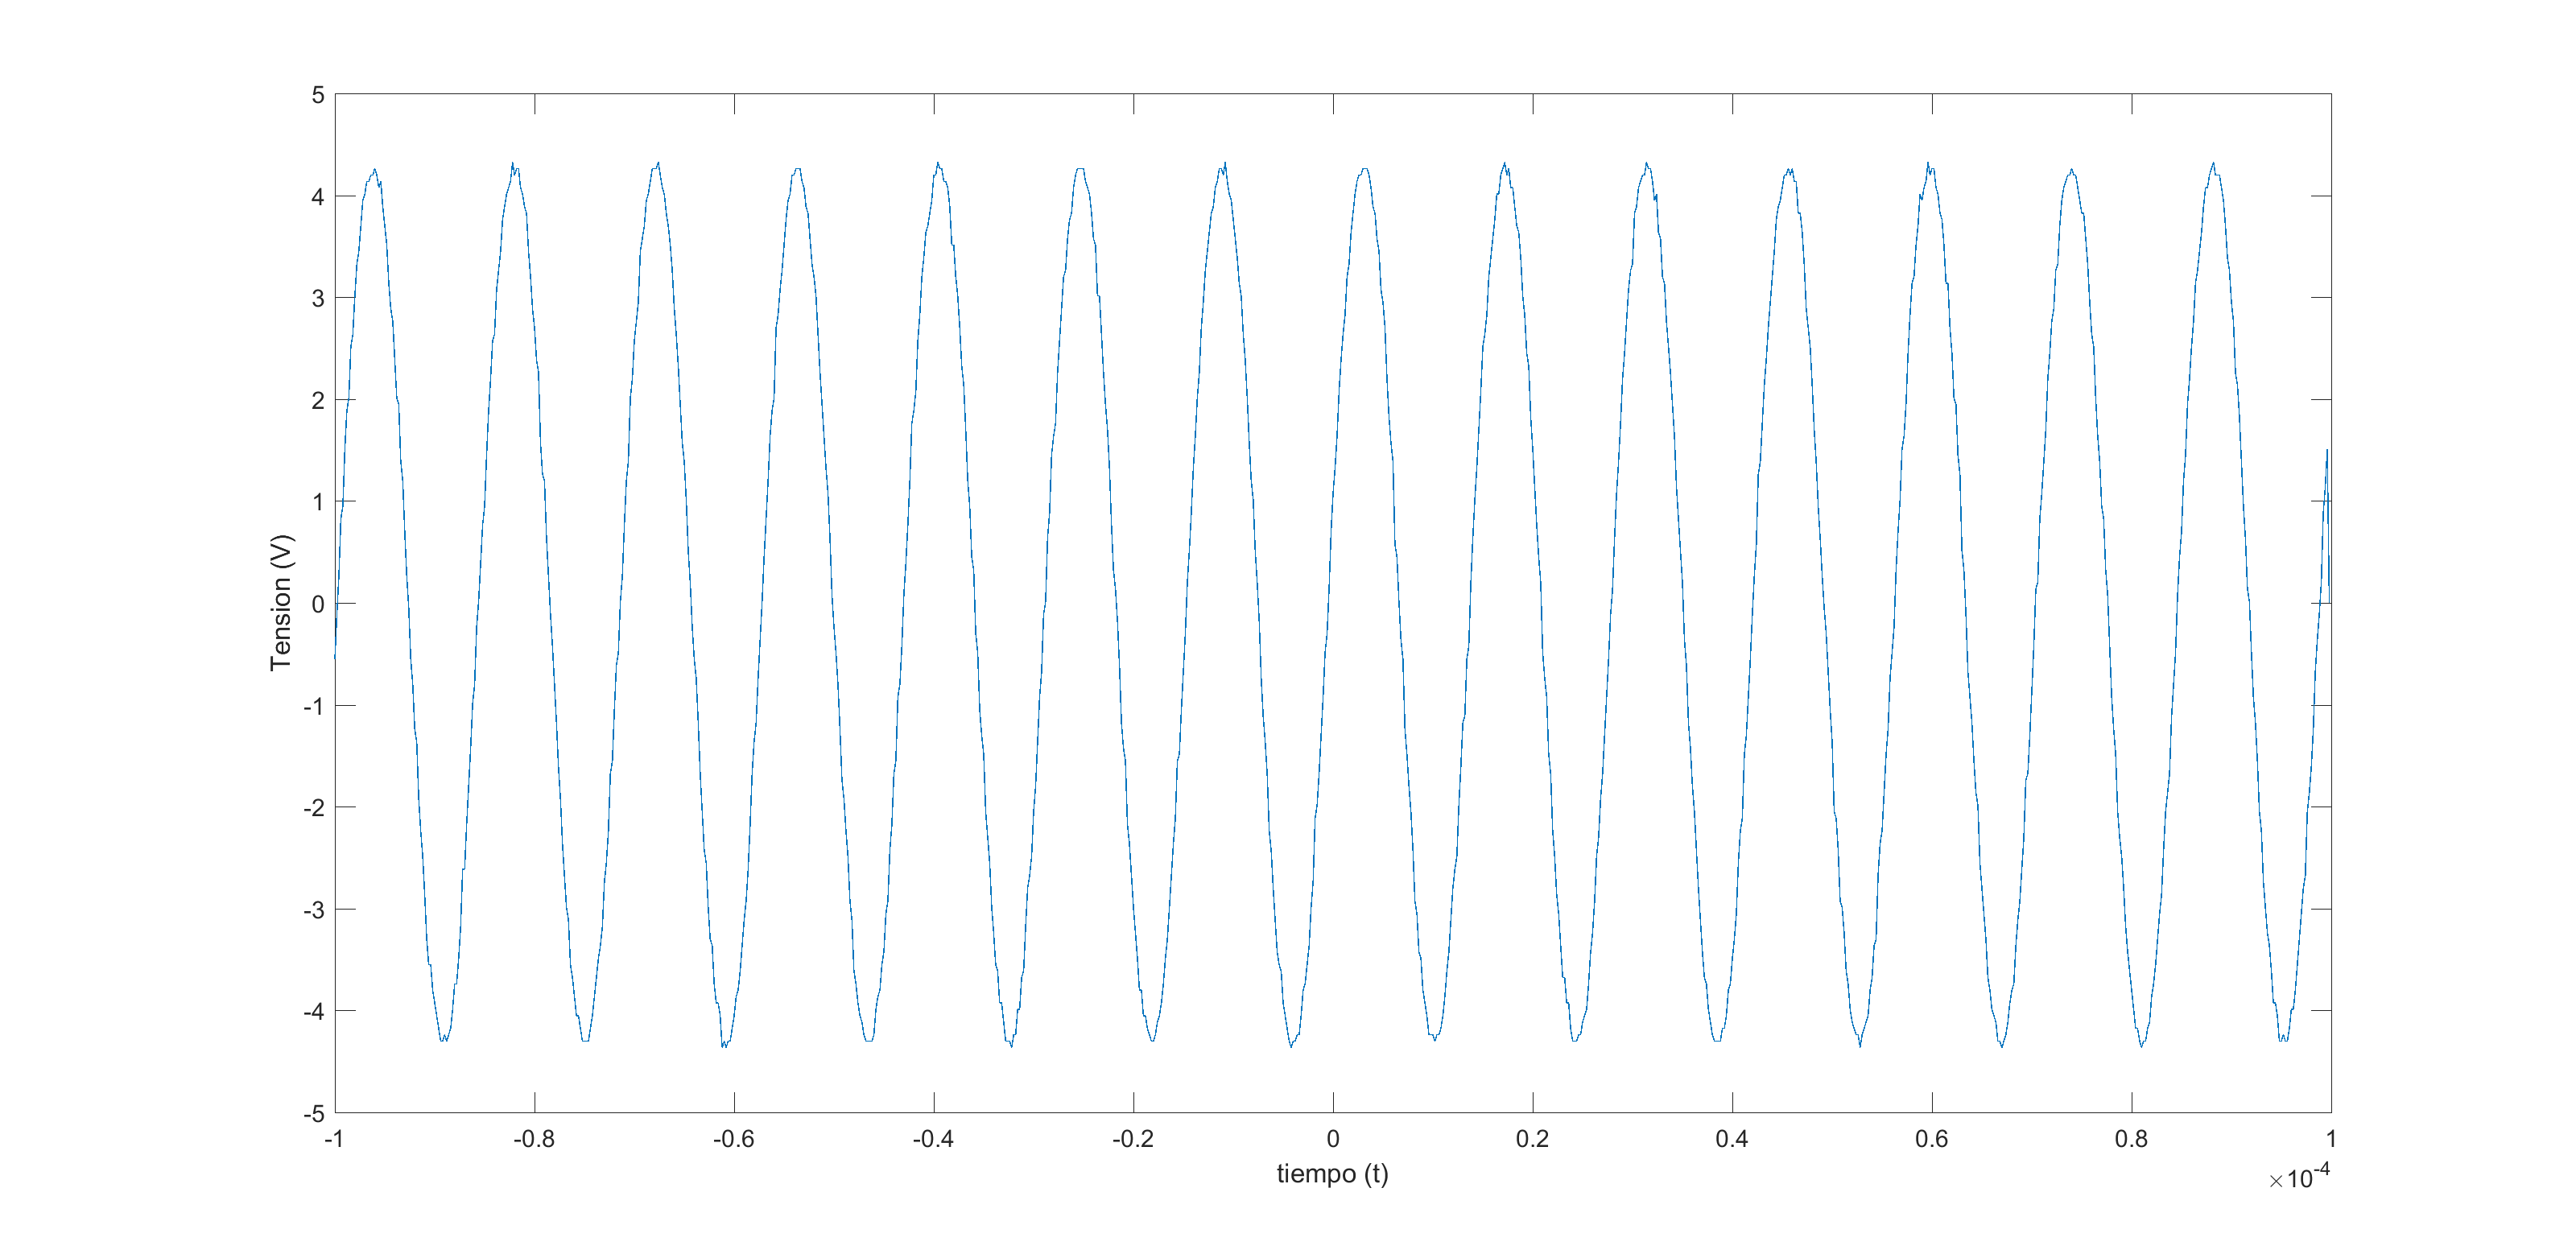
\includegraphics[scale=0.2]{imagenes/oscilacion.png}
	\caption{Oscilación resultante con el oscilador de Wien ya implementado}
	\label{fig:ej1_oscilacion}
\end{figure}
Que arrojó una frecuencia de 70.2kHz, con una tensión pico de aproximadamente 4.2V.

\subsection{Distorsión Armónica}
Se utilizó el osciloscopio para observar el espectro en frecuencia de la señal generada. Se utilizó entonces la función FFT, configurada en Blackman Harris, con un scope de 1Mhz.
Se observó entonces el siguiente espectro: 

\begin{figure}[H]	
	\centering
	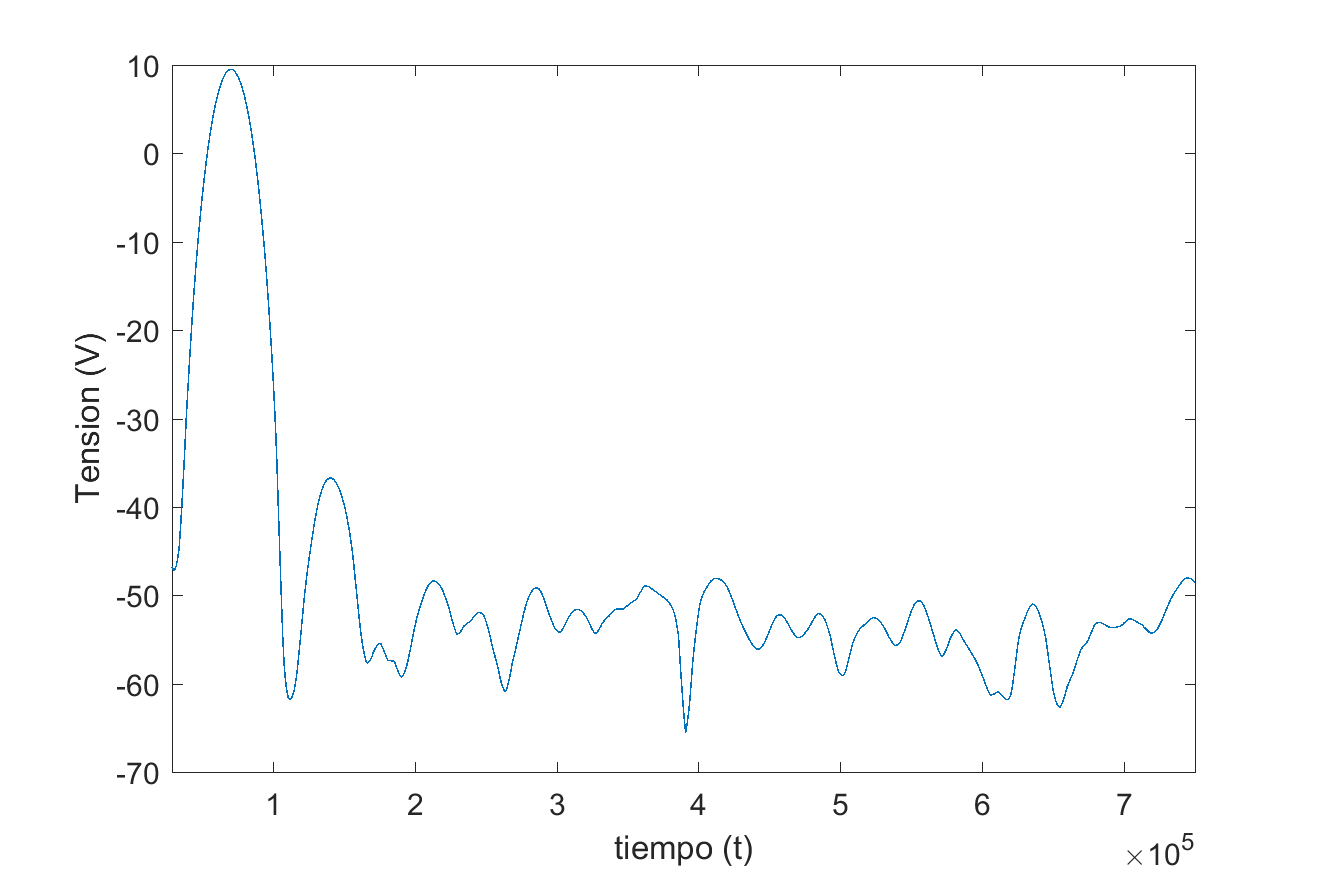
\includegraphics[scale=0.5]{imagenes/fft_armonicos.png}
	\caption{Espectro de la señal incluyendo 10 armónicos}
	\label{fig:ej1_fft_armonicos}
\end{figure}

Del cual se obtuvo la siguiente tabla de datos para obtener el THD de la señal generada, utilizando la fórmula $THD = \frac{P_{armonicos}}{P_{total}}$, donde P es la potencia calculada con la FFT para determinada frecuencia: 

	\begin{table}[H] %datos thd simulado
				\centering
 				\begin{tabular}{||c c||} 
 					\hline
					$frecuencia(kHz)$ & Potencia(dB)\\ [0.5ex] 
 					\hline\hline
					70.2 & $10.03$\\
					140.3 & $-28.15$\\
					210.5 & $-32.5$\\
					280.6 & $-49.17$\\
					350.8 & $-41.5$\\
					420 & $-44.33$\\
					491.1 & $-56,06$\\
					561,5 & $-49,5$\\
					631.45 & $-56.89$\\
					701.59 & $-57.09$\\[1ex] 
					\hline
				\end{tabular}
			\end{table}
\end{document}
